% Created 2020-03-25 qua 12:05
% Intended LaTeX compiler: pdflatex
\documentclass[11pt]{article}
\usepackage[utf8]{inputenc}
\usepackage[T1]{fontenc}
\usepackage{graphicx}
\usepackage{grffile}
\usepackage{longtable}
\usepackage{wrapfig}
\usepackage{rotating}
\usepackage[normalem]{ulem}
\usepackage{amsmath}
\usepackage{textcomp}
\usepackage{amssymb}
\usepackage{capt-of}
\usepackage{hyperref}
\usepackage[newfloat, cache = false]{minted}
\usepackage{amsmath}
\usepackage{amsthm}
\usepackage{tikz}
\usetikzlibrary{positioning}
\usepackage{subfigure}
\newtheorem{exercicio}{Exercício}
\newtheorem{theorem}{Teorema}
\author{Luiz Alberto do Carmo Viana}
\date{\today}
\title{Estruturas de Dados}
\hypersetup{
 pdfauthor={Luiz Alberto do Carmo Viana},
 pdftitle={Estruturas de Dados},
 pdfkeywords={},
 pdfsubject={},
 pdfcreator={Emacs 26.3 (Org mode 9.3.6)}, 
 pdflang={English}}
\begin{document}

\maketitle
\begin{abstract}
Notas de aula para as disciplinas de Estrutura de Dados e Estrutura de Dados Avançada do curso de Ciência da Computação do campus da UFC em Crateús.
\end{abstract}

\setcounter{tocdepth}{2}
\tableofcontents

\pagebreak

\section{Introdução}
\label{sec:org50d9085}

Logo após os conceitos básicos de programação, é necessário aprender
a escrever programas que façam um bom uso dos recursos do
computador.  Tais recursos consistem, dentre outros, das unidades de
processamento e das unidades de armazenamento.

Em se tratando de armazenamento, ou mais precisamente da memória do
computador, é sabido que boa parte da execução de um programa
consiste em obter dados que devem ser, de alguma forma, processados.
Nota-se, portanto, que o custo de execução de um programa não
depende apenas do tempo de processamento dos dados, mas também do
tempo de acesso a eles.

Nestas notas de aula, vamos lidar com boas práticas para a
organização e gerenciamento dos dados na memória do computador.  Com
elas, nossos programas podem armazenar, e portanto acessar, de forma
eficiente os dados que produzem ou recebem de seus usuários.

Para descrever e implementar nossas estruturas de dados, vamos
utilizar a linguagem \texttt{C++}, em seu padrão \texttt{C++17}.  Construiremos
nossos programas com as ferramentas de compilação do projeto GNU, em
particular o compilador \texttt{g++} e o \emph{build manager} \texttt{make}.

\subsection{Ferramentas}
\label{sec:org720ef4b}

Primeiro, descrevemos como vamos utilizar o programa \texttt{make}.
Para isso, vamos explicar o que é um arquivo \texttt{makefile} e,
aos poucos, o conteúdo do nosso.

O arquivo \texttt{makefile} descreve como um projeto deve ser
construído, e costuma situar-se no diretório raiz de seu projeto.
Seu conteúdo consiste de variáveis e regras.  Cada regra determina,
por meio de uma ``receita'', como um alvo deve ser construído a
partir de seus pré-requisitos.  Vale notar que um alvo pode ser
pré-requisito de outros alvos, o que permite uma abordagem
hierárquica para a construção de um projeto.

Vamos enumerar o conteúdo de nosso \texttt{makefile}, a começar por
suas variáveis.

\begin{minted}[,fontsize=\footnotesize]{makefile}
# compiler and c++ standard variables
COMPILER = g++
STD      = c++17
\end{minted}

Começamos criando duas variáveis, com o propósito de determinar, de
maneira flexível, o compilador que vamos utilizar junto com o
padrão da linguagem.  Vamos fazer uso dessas variáveis para a
construção de comandos.  Observamos também que linhas comentadas
devem ser iniciadas com \texttt{\#}.

\begin{minted}[,fontsize=\footnotesize]{makefile}
# directories to look for .h and .hpp files (preceded by -I parameter)
INCLUDE_DIRS = -I.
\end{minted}

Com a variável \texttt{INCLUDE\_DIRS}, listamos os diretórios em
que vamos buscar por arquivos-cabeçalho.  Como vamos utilizar essa
informação em chamadas do compilador, precedemos o nome de cada
diretório por \texttt{-I}.  No presente momento, indicamos que
apenas o diretório raiz do projeto (\texttt{.}) contém
arquivos-cabeçalho de nosso interesse.

\begin{minted}[,fontsize=\footnotesize]{makefile}
# compiler parameters for compiling and linking
COMPILING_OPTIONS = -c -g -std=$(STD) $(INCLUDE_DIRS) -Wall -Wextra
LINKING_OPTIONS   = -g -std=$(STD) -Wall -Wextra
\end{minted}

Definimos a variável \texttt{COMPILING\_OPTIONS} com os parâmetros
a serem utilizados na fase de compilação.  Observe a utilização das
variáveis \texttt{STD} e \texttt{INCLUDE\_DIRS}, definidas
anteriormente. Para a fase de \emph{linking}, usamos os parâmetros
definidos em \texttt{LINKING\_OPTIONS}.

\begin{minted}[,fontsize=\footnotesize]{makefile}
# list of project headers
HEADERS = bstree.hpp avltree.hpp rbtree.hpp
\end{minted}

A variável \texttt{HEADERS} lista os arquivos-cabeçalho que
utilizaremos nestas notas de aula.  Cada um desses arquivos deve
conter as definições de exatamente uma estrutura de dados.
Utilizaremos a extensão \texttt{.hpp}, uma vez que nossas classes
terão seus métodos definidos diretamente em sua declaração.

\begin{minted}[,fontsize=\footnotesize]{makefile}
# these variables define one tester program for each header
TESTERS_SRC = $(HEADERS:.hpp=_test.cpp)
TESTERS_OBJ = $(TESTERS_SRC:.cpp=.o)
TESTERS     = $(TESTERS_SRC:.cpp=)
\end{minted}

Como é boa prática em programação, vamos definir um programa
testador para cada uma de nossas estruturas de dados.  Com a
decisão de conter exatamente uma estrutura de dados por arquivo
\texttt{.hpp}, basta haver um testador para cada cabeçalho.

A variável \texttt{TESTERS\_SRC} determina justamente isso: para
cada entrada em \texttt{HEADERS}, trocamos o sufixo \texttt{.hpp}
por \texttt{\_test.cpp}.  De forma similar, a variável
\texttt{TESTERS\_OBJ} traz os nomes dos arquivos-objeto de nossos
programas testadores, assim como \texttt{TESTERS} indica o nome de
seus arquivos executáveis.  Note o truque empregado em
\texttt{TESTERS} para excluir a extensão \texttt{.cpp} dos nomes em
\texttt{TESTERS\_SRC}.  Agora, vamos começar a descrever algumas
``receitas''.

\begin{minted}[,fontsize=\footnotesize]{makefile}
# $< refers to prerequisite and $@ refers to target name

# instructions for creating object files from cpp files
%.o : %.cpp
     $(COMPILER) $(COMPILING_OPTIONS) $< -o $@
\end{minted}

Em nossa primeira ``receita'', determinamos como deve ser obtido um
arquivo-objeto qualquer (\texttt{\%.o}) a partir de seu arquivo
\texttt{.cpp} correspondente (\texttt{\%.cpp}).  A primeira linha
significativa de nossa ``receita'' é da forma
\texttt{target : prerequisites}, estabelecendo a relação de
dependência entre arquivos \texttt{.o} e arquivos \texttt{.cpp}.
As demais linhas, que devem ser indentadas com \texttt{TAB},
constituem os comandos necessários para a criação do alvo.  Nesse
caso, temos apenas um comando, criado a partir de variáveis que
definimos anteriormente. Também fazemos uso de duas variáveis
especiais: \texttt{\textbackslash{}\$@} refere-se ao nome do alvo, e \texttt{\textbackslash{}\$<}
ao nome do primeiro pré-requisito (para os nomes de todos os
pré-requisitos, podemos usar \texttt{\textbackslash{}\$\textbackslash{}\textasciicircum{}}).

\begin{minted}[,fontsize=\footnotesize]{makefile}
# instructions for creating tester programs and running them
%_test : %_test.o %.hpp
     $(COMPILER) $(LINKING_OPTIONS) $< -o $@
     ./$@
\end{minted}

Agora apresentamos a ``receita'' responsável por criar os
executáveis testadores e executá-los.  Dessa vez, utilizamos dois
comandos: criamos o executável, que em seguida é utilizado.

\begin{minted}[,fontsize=\footnotesize]{makefile}
# this indicates that these rules do not correspond to files
.PHONY : test clean
\end{minted}

Esse trecho do \texttt{makfile} serve para indicar que as
``receitas'' \texttt{test} e \texttt{clean} não correspondem a
nomes de arquivos (\emph{phony} significa falso).  Isso é útil para
definirmos as formas como vamos invocar o programa \texttt{make}.

\begin{minted}[,fontsize=\footnotesize]{makefile}
# instructions on how to clean the project (deleting some stuff)
clean :
     rm -f *.o
     rm -f $(TESTERS)
\end{minted}

A ``receita'' \texttt{clean} tem a finalidade de remover arquivos
intermediários ou auxiliares.  Note que ela não tem pré-requisitos
e usa dois comandos, deletando arquivos-objeto e programas
testadores.

\begin{minted}[,fontsize=\footnotesize]{makefile}
# this runs the test suite
test : $(TESTERS)
\end{minted}

Por último, a ``receita'' \texttt{testers} executa todos os
programas testadores que foram modificados desde sua última
execução.  Observe que, como seu propósito é apenas agrupar a
execução de vários programas em uma única instrução, não é
necessário que \texttt{test} tenha comandos próprios.

\pagebreak

\section{Estruturas de Dados Arbóreas}
\label{sec:org9625186}

Vamos começar nosso estudo com Árvores Binárias de Busca simples,
sem balanceamento.  Em seguida, vamos apresentar técnicas que
garantem uma boa distribuição de altura entre sub-árvores.  Por fim,
analisamos árvores que permitem mais de dois filhos por nó.

\subsection{Árvores Binárias de Busca}
\label{sec:org575f560}

\subsubsection{Introdução}
\label{sec:orge319958}

TODO escrever isso apenas ao lecionar Estruturas de Dados.

\subsubsection{Implementação}
\label{sec:org7207aa6}

Vamos criar o arquivo \texttt{bstree.hpp} para conter a declaração de uma
classe que implementa, de forma genérica, o conceito de Árvore
Binária de Busca. Junto a ela, estarão as definições de seus
métodos, cada um correspondendo a uma operação simples: busca,
inserção, e remoção.

\begin{minted}[,fontsize=\footnotesize]{c++}
// each compilation session must consider this file at most once
#pragma once

// we are going to use smart pointer facilities
#include <memory>
// this type is helpful to represent optional value returning
#include <optional>
\end{minted}

Começamos \texttt{bstree.hpp} com algumas diretivas de pré-processamento.
A declaração \texttt{\#pragma once} determina que o código-fonte contido
no arquivo deve ser avaliado uma única vez em cada sessão de
compilação.  Em seguida, temos dois \texttt{\#include}: \texttt{<memory>} vai nos
dar acesso aos ponteiros inteligentes de \texttt{C++}, automatizando o
gerenciamento de memória; \texttt{<optional>} define um tipo genérico
contendo zero ou um elementos de um certo tipo.

\begin{minted}[,fontsize=\footnotesize]{c++}
// generic types
template<typename Key, typename Val>
class BSTree{
  // ...
};
\end{minted}

Definimos a classe \texttt{BSTree}, com algo que pode ser novo para o
leitor.  A linha de \texttt{template} cria dois símbolos, \texttt{Key} e \texttt{Val},
que serão usados, dentro de \texttt{BSTree}, para representar os tipos de
chave e valor, respectivamente, a serem armazenados (em pares) nos
nós de nossa \texttt{BSTree}.  Isso nos permite declarar, por exemplo,
uma \texttt{BSTree} que mapeia valores inteiros a strings com
\texttt{BSTree<int, std::string>}.  Vamos agora preencher o conteúdo
dessa classe.

\begin{minted}[,fontsize=\footnotesize]{c++}
// ...
private:
  // node of BSTree
  class BSTreeNode{
  // ...
  };

  // root node of BSTree
  std::unique_ptr<BSTreeNode> root;
// ...
\end{minted}

Primeiro, falamos dos membros privados de \texttt{BSTree}.  A classe
aninhada \texttt{BSTreeNode} (a ser definida futuramente) é responsável
por representar um nó de nossa \texttt{BSTree}, junto com algumas
operações.  O outro membro privado é um ponteiro inteligente cuja
função é referenciar o nó raiz de nossa \texttt{BSTree}.

Um ponteiro \texttt{unique\_ptr} traz a garantia de ser o único ponteiro
inteligente que referencia um certo endereço de memória.  Assim,
vemos que é razoável \texttt{root} ser do tipo
\texttt{std::unique\_ptr<BSTreeNode>}, afinal, para preservar as
propriedades de instâncias de nossa estrutura de dados, é saudável
que apenas elas tenham acesso a suas respectivos raizes.

\begin{minted}[,fontsize=\footnotesize]{c++}
// ...
public:
  // constructor to create an empty BSTree
  BSTree() : root{nullptr}
  {}

  // constructor to create a BSTree rooted by Key and Val
  BSTree(Key key, Val val) : root{std::make_unique<BSTreeNode>(key, val)}
  {}

  // ...
\end{minted}

Como nossos primeiros membros públicos, apresentamos dois
construtores para \texttt{BSTree}.  Em \texttt{C++}, construtores têm, além de
um corpo (a sequência de instruções delimitadas por chaves), uma
lista de inicialização para as variáveis-membro de sua classe.

O primeiro construtor não recebe argumentos e cria uma \texttt{BSTree}
vazia, com \texttt{root} assumindo o valor \texttt{nullptr}.  Já o segundo
construtor, que recebe valores de tipos \texttt{Key} e \texttt{Val}, deve criar
o nó raiz de sua instância, e para isso utiliza a função
\texttt{make\_unique}.  Observe que ambos têm um corpo vazio.

\begin{minted}[,fontsize=\footnotesize]{c++}
// ...
public:
  // ...

  bool isEmpty(){
    return root == nullptr;
  }

  // returns Key Val pair whose Val corresponds to the maximum BSTree
  // Key
  std::optional<std::pair<Key, Val>> maxKey(){
    if (root){
      return root->maxKey();
    }
    else{
      return {};
    }
  }

  // returns Key Val pair whose Val corresponds to the minimum BSTree
  // Key
  std::optional<std::pair<Key, Val>> ninKey(){
    if (root){
      return root->minKey();
    }
    else{
      return {};
    }
  }

  // ...
\end{minted}

Aqui temos mais três métodos públicos.  Não há tanta necessidade
de explicar \texttt{isEmpty}, dada sua simplicidade.

Note que \texttt{maxKey} e \texttt{minKey} retornam valores de mesmo
tipo. Utilizamos \texttt{std::pair<Key, Val>} para declarar um par cuja
primeira (segunda) componente tem um valor de tipo \texttt{Key}
(\texttt{Val}). Além disso, fazemos uso do tipo
\texttt{std::optional<std::pair<Key, Val>>} para indicar que os métodos
retornam um objeto que pode conter um par ou nada.  Caso a
\texttt{BSTree} não esteja vazia, ambos delegam seu retorno para métodos
homônimos de \texttt{BSTreeNode}.

\pagebreak

\begin{minted}[,fontsize=\footnotesize]{c++}
// ...
public:
  // ...

  // searches for Key, returning the corresponding Value or nothing
  std::optional<Val> search(Key key){
    if (root){
      return root->search(key);
    }
    else{
      return {};
    }
  }

  // inserts Val attached to Key in case Key is not present
  // yet. Return value indicates whether insertion really took place
  bool insert(Key key, Val val){
    if (root){
      return root->insert(key, val);
    }
    else{
      root = std::make_unique<BSTreeNode>(key, val);
      return true;
    }
  }

  // removes Key and corresponding attached Val. Return value
  // indicates whether removal really took place
  bool remove(Key key){
    // ...
  }
\end{minted}

Agora temos as três operações principais em \texttt{BSTree}.  Por hora,
vamos definir \texttt{search} e \texttt{insert}, ambos delegando sua operação
para métodos homônimos de \texttt{BSTreeNode} caso \texttt{BSTree} não esteja
vazia.

É digno de nota que \texttt{search} e \texttt{insert} usam seus retornos para
indicar se a operação foi bem-sucedida ou não.  Em \texttt{insert}, é
retornado \texttt{false} sse a chave a ser inserida já está presente na
\texttt{BSTree}.  Já em \texttt{search}, usa-se \texttt{std::optional<Val>} para
permitir que se retorne nada caso a chave buscada não esteja
presente na \texttt{BSTree}. Definimos agora a classe \texttt{BSTreeNode}.

\pagebreak

\begin{minted}[,fontsize=\footnotesize]{c++}
class BSTreeNode{
public:
  // since this is an internal private class, there is no need to
  // private members
  Key key;
  Val val;
  // smart pointers to left and right subtrees: these guys deal with
  // memory deallocation by themselves
  std::unique_ptr<BSTreeNode> left;
  std::unique_ptr<BSTreeNode> right;

  // ...
};
\end{minted}

Como se trata de uma classe aninhada privada, não existe a
necessidade de declarar seus membros como privados.  Como
variáveis, \texttt{BSTreeNode} armazena um par de chave e valor, além de
ponteiros inteligentes para suas sub-árvores esquerda e diretia.
Como descrevem os comentários, ponteiros inteligentes são capazes
de lidar com a desalocação de memória.

\pagebreak

\begin{minted}[,fontsize=\footnotesize]{c++}
// ...
public:
  // ...

  // constructor: notice that member initialization is done outside
  // of the constructor body
  BSTreeNode(Key k, Val v) : key{k},
                             val{v},
                             left{nullptr},
                             right{nullptr}
  {}

  // returns Key Val pair whose Key is maximum
  std::pair<Key, Val> maxKey(){
    if (right){
      return right->maxKey();
    }
    else{
      return std::make_pair(key, val);
    }
  }

  // returns Key Val pair whose Key is minimum
  std::pair<Key, Val> minKey(){
    if (left){
      return left->minKey();
    }
    else{
      return std::make_pair(key, val);
    }
  }

  // ...
\end{minted}

Não há nada novo no único construtor de \texttt{BSTreeNode}.  Já os
métodos \texttt{minKey} e \texttt{maxKey} valem-se das invariantes de \texttt{BSTree}
para retornar apropriadamente.

Como a chave de um nó de \texttt{BSTree} é menor que a de qualquer nó em
sua sub-árvore direita, ela é mínima sse sua sub-árvore esquerda é
vazia.  Em caso negativo, buscamos a chave mínima da sub-árvore
esquerda.  Isso justifica a corretude de \texttt{minKey}, e um argumento
análogo se aplica a \texttt{maxKey}.

\pagebreak

\begin{minted}[,fontsize=\footnotesize]{c++}
// ...
public:
  // ...

  // searches for Key, returning a Val or nothing
  std::optional<Val> search(Key k){
    // current node contains requested key
    if (k == key){
      return val;
    }
    // left subtree is not empty and requested key may be at it
    else if (left && k < key){
      return left->search(k);
    }
    // the same in regard of right subtree
    else if (right && k > key){
      return right->search(k);
    }
    // if requested key cannot be found, return nothing
    return {};
  }

  // ...
\end{minted}

O método \texttt{search} recebe como argumento um valor do tipo \texttt{Key} e
talvez retorne um valor do tipo \texttt{Val}, encapsulado em \texttt{optional}.
Em \texttt{search}, vemos o uso das invariantes de \texttt{BSTree} na condução
da busca por \texttt{k}: caso \texttt{k} não seja a raiz do nó atual, deve-se
buscar por \texttt{k} na sub-árvore direita ou esquerda, a depender de
como \texttt{k} se compara com \texttt{key} e se a devida sub-árvore é
não-vazia.

\pagebreak

\begin{minted}[,fontsize=\footnotesize]{c++}
// ...
public:
  // ...

  // inserts Val attached to Key in case Key is not present. Return
  // value indicates whether insertion really happened
  bool insert(Key k, Val v){
    // current node already contains Key, so does nothing
    if (k == key){
      return false;
    }
    // insertion may occur at left subtree
    else if (k < key){
      // if left subtree is not empty, recursively inserts into it
      if (left){
        return left->insert(k, v);
      }
      // if left subtree is empty, insertion will occur
      else{
        left = std::make_unique<BSTreeNode>(k, v);
      }
    }
    // same idea but applied to right subtree
    else if (k > key){
      if (right){
        return right->insert(k, v);
      }
      else{
        right = std::make_unique<BSTreeNode>(k, v);
      }
    }
    // if execution reaches this line, insertion indeed has occured,
    // so returns accordingly
    return true;
  }
\end{minted}

No método \texttt{insert}, mais uma vez as invariantes de \texttt{BSTree} ficam
evidentes.  Caso a inserção seja conduzida para uma sub-árvore
vazia, ela de fato ocorre, criando o primeiro nó daquela
sub-árvore. Caso a sub-árvore não esteja vazia, a inserção é
tentada recursivamente.  Enfim definimos \texttt{remove}.

\pagebreak

\begin{minted}[,fontsize=\footnotesize]{c++}
bool remove(Key key){
  // if BSTree is not empty, we may have something to delete
  if (root){
    // ...
  }
  // if BSTree is empty, we simply indicate nothing was deleted
  else{
    return false;
  }
}
\end{minted}

A primeira coisa que \texttt{remove} verifica é se a árvore está vazia.
Em caso afirmativo, nada vai ser removido e o retorno indica isso.

\begin{minted}[,fontsize=\footnotesize]{c++}
if (root){
  // raw pointers to perform a traversal
  BSTreeNode* currentNode = root.get();
  // since currentNode starts pointing towards root, it has no
  // parent node
  BSTreeNode* parentNode  = nullptr;
  // tries to find requested key. This may end up in an empty
  // subtree
  while (currentNode && key != currentNode->key){
    // updates parentNode
    parentNode = currentNode;
    // goes either left or right accordingly
    if (key < currentNode->key){
      currentNode = currentNode->left.get();
    }
    else if (key > currentNode->key){
      currentNode = currentNode->right.get();
    }
  }

  // ...
}
\end{minted}

Caso a árvore não esteja vazia, fazemos uma ``descida'' em sua
estrutura, buscando pela chave a ser removida.  Para isso, usamos
ponteiros simples \texttt{currentNode} e \texttt{parentNode} cujo propósito é
indicar, respectivamente, o nó atual e seu pai.  Como nossa busca
começa pela raiz, \texttt{parentNode} é inicialmente nulo.

Vale observar que, apesar de estarmos usando o método \texttt{get} de um
ponteiro inteligente para ter acesso ao ponteiro simples que ele
encapsula, não seria boa prática desalocar a região referenciada
pelo ponteiro simples (com \texttt{delete} ou \texttt{free}), uma vez que essa
responsabilidade é atribuída ao ponteiro inteligente. Isso quer
dizer que, no momento de destruição do ponteiro inteligente, a
região de memória por ele referenciada será invariavelmente
desalocada, e caso já o tenha sido, teremos um \emph{double free
error}.  Assim, usamos ponteiros simples apenas para ``passear''
pela estrutura, e nenhum gerenciamento de memória os compete.

O laço \texttt{while} apresentado faz \texttt{currentNode} ``descer''
apropriadamente na estrutura da árvore sempre que a chave buscada
é diferente de sua chave.  Além disso, \texttt{parentNode} mantém o valor
anterior de \texttt{currentNode}.

\begin{minted}[,fontsize=\footnotesize]{c++}
if (root){
  // ...

  // now we must verify why we exited the while loop
  // if currentNode is not nullptr, we exited the while loop
  // because key == currentNode->key, so currentNode content must
  // be deleted
  if (currentNode){
    // ...
  }
  // if currentNode is nullptr, then the only subtree that could
  // contain key is empty, so no deletion is performed
  else{
    return false;
  }
}
\end{minted}

Uma vez fora do \texttt{while}, é preciso verificar que parte de sua
condição foi violada.  Caso a saída tenha ocorrido por conta de
\texttt{currentNode} assumir um valor nulo, então a ``descida'' em busca
da chave a ser removida nos levou a uma sub-árvore vazia, o que
indica que a chave que buscávamos não existia na árvore.

\begin{minted}[,fontsize=\footnotesize]{c++}
if (currentNode){
  // currentNode has no subtrees, so it can safely be deleted
  if (currentNode->left == nullptr && currentNode->right == nullptr){
    // ...
  }
  // currentNode has both subtrees not empty
  else if (currentNode->left && currentNode->right){
    // ...
  }
  // currentNode has exactly one subtree not empty
  else{
    // ...
  }

  return true;
}
\end{minted}

Agora que vamos de fato lidar com a remoção de um nó da árvore,
nos deparamos com três cenários possíveis: o nó não tem
sub-árvores significativas, e portanto pode ser simplesmente
excluído; o nó tem ambas as suas sub-árvores não-vazias; o nó tem
exatamente uma sub-árvore não vazia, e esta vai ocupar o seu
lugar.  Vamos tratar cada um desses casos.

\begin{minted}[,fontsize=\footnotesize]{c++}
if (currentNode->left == nullptr && currentNode->right == nullptr){
  // currentNode is not root
  if (parentNode){
    // ...
  }
  // currentNode is root, so we simply deallocate BSTreeNode
  // at root
  else{
    root = nullptr;
  }
}
\end{minted}

Caso o nó não tenha sub-árvores significativas, podemos
removê-lo. Contudo, precisamos verificar se ele é a raiz da
árvore, pois nesse caso é preciso atualizar \texttt{root}.  Note ainda
que, como \texttt{root} é um \texttt{unique\_ptr}, \texttt{root} não perde sua
referência sem antes desalocá-la (isso pode ser feito de forma
segura, dado que um \texttt{unique\_ptr} mantém uma referência de forma
exclusiva).  Assim, atribuir \texttt{nullptr} a \texttt{root} é o suficiente.

\begin{minted}[,fontsize=\footnotesize]{c++}
if (parentNode){
  // currentNode is parentNode's left child
  if (currentNode->key < parentNode->key){
    // this assignment is enough to deallocate currentNode
    parentNode->left = nullptr;
  }
  // currentNode is parentNode's right child
  else if (currentNode->key >  parentNode->key){
    parentNode->right = nullptr;
  }
}
\end{minted}

Quando o nó não é a raiz da árvore, precisamos verificar como ele
se relaciona com seu pai.  Assim, podemos determinar qual filho de
\texttt{parentNode} deve ser removido.  Note ainda que \texttt{parentNode->left}
e \texttt{parentNode->right} são do tipo \texttt{unique\_ptr}.  Vamos para o
próximo cenário de remoção.

\pagebreak

\begin{minted}[linenos,firstnumber=1,fontsize=\footnotesize]{c++}
else if (currentNode->left && currentNode->right){
  // we could also have taken currentNode->right->minKey
  auto[leftMaxKey, leftMaxVal] = currentNode->left->maxKey();

  remove(leftMaxKey);

  currentNode->key = leftMaxKey;
  currentNode->val = leftMaxVal;
}
\end{minted}

No caso em que o nó a ser deletado tem ambas as sub-árvores
não-vazias, curiosamente não é ele quem é removido.  Em vez disso,
tomamos o conteúdo do nó com a maior chave em sua sub-árvore
esquerda e ``copiamos'' esse conteúdo no nó que deveria ser
removido. Isso faz com que o conteúdo que deveria ser deletado de
fato desapareça da árvore, e nos permite remover um nó com ao
menos uma sub-árvore vazia.

\begin{exercicio}
O que aconteceria caso \texttt{remove(leftMaxkey);} fosse posta como a
última instrução em seu bloco?
\end{exercicio}

\begin{exercicio}
Por que o nó de \texttt{leftMaxkey} tem ao menos uma sub-árvore vazia?
\end{exercicio}

Precisamos ainda destacar uma novidade sintática. Como o método
\texttt{maxKey} de \texttt{BSTreeNode} retorna um valor do tipo \texttt{std::pair<Key,
    Val>}, podemos receber esse retorno de forma desestruturada, isto
é, atribuindo separadamente os valores de tipos \texttt{Key} e \texttt{Val} a
variáveis recém-criadas.  É precisamente esse o propósito da
sintaxe utilizada na linha 3 da última
listagem.

\begin{minted}[,fontsize=\footnotesize]{c++}
else{
  // currentNode is not root
  if (parentNode){
    // ..
  }
  // currentNode is root, so we update root to be its only
  // nonempty subtree
  else{
    if (currentNode->left){
      root = std::move(currentNode->left);
    }
    else if (currentNode->right){
      root = std::move(currentNode->right);
    }
  }
}
\end{minted}

Agora lidamos com o caso em que o nó a ser removido tem exatamente
uma sub-árvore não-vazia.  Nesse cenário, o nó pode ser
desalocado, com sua única sub-árvore não-vazia agora referenciada
por seu pai.

Mais uma vez, devemos fazer a distinção se o nó a ser removido é a
raiz da árvore ou não. Caso seja, apenas sobrescrevemos \texttt{root} com
a referência de sua única sub-árvore não-vazia.

Destacamos o uso de \texttt{std::move}.  Em \texttt{C++} moderno, podemos tanto
``copiar'' como ``recortar'' variáveis.  Para ``copiar'' uma
variável, basta uma operação de atribuição.  Já para ``cortar'',
passamos a variável a ser ``cortada'' como argumento para
\texttt{std::move} durante a operação de atribuição. Assim, após \texttt{a =
    std::move(b)}, o conteúdo de \texttt{b} deve estar em \texttt{a}, e acessar \texttt{b}
pode ter comportamento indefinido, portanto não é recomendado.

\begin{exercicio}
Pesquise sobre \emph{move semantics} em \texttt{C++}.
\end{exercicio}

Posto isso, perceba que não faz muito sentido ``copiar'' o
conteúdo de um \texttt{unique\_ptr}, já que haveriam ao menos dois deles
apontando para um mesmo endereço.  Inclusive, tentar fazer isso
resultaria em um erro de compilação.  No nosso caso, de fato
queremos ``cortar'' a sub-árvore não-vazia de \texttt{root} e atribuí-la
a \texttt{root}.

\begin{minted}[,fontsize=\footnotesize]{c++}
if (parentNode){
  // currentNode is parentNode's left child
  if (currentNode->key < parentNode->key){
    if (currentNode->left){
      // notice how we don't copy the unique_ptr. We move it
      // instead
      parentNode->left = std::move(currentNode->left);
    }
    else if (currentNode->right){
      parentNode->left = std::move(currentNode->right);
    }
  }
  // currentNode is parentNode's right child
  else if (currentNode->key > parentNode->key){
    if (currentNode->left){
      parentNode->right = std::move(currentNode->left);
    }
    else if (currentNode->right){
      parentNode->right = std::move(currentNode->right);
    }
  }
}
\end{minted}

Caso o nó a ser removido não seja a raiz da árvore, atualizamos a
sub-árvore apropriada de \texttt{parentNode}.  Mais uma vez, precisamos
determinar qual a única sub-árvore não-vazia de \texttt{currentNode}.

\subsubsection{Análise de Complexidade}
\label{sec:org3e62ace}

TODO escrever isso apenas ao lecionar Estruturas de Dados.

\begin{exercicio}
Prove que, se um nó em uma Árvore Binária de Busca tem dois
filhos, então seu sucessor não tem filho esquerdo e seu antecessor
não tem filho direito.
\end{exercicio}

\subsection{Árvores AVL}
\label{sec:orgd5f0094}
\label{org6ea5e87}

Sabendo que as operações de busca, inserção e remoção de uma Árvore
Binária de Busca têm complexidade \(O(h)\), onde \(h\) é a altura da
árvore, devemos fazer suas operações de modificação de forma a
minimizar a altura da árvore resultante.  Com esse objetivo, vamos
definir o conceito de Árvore AVL, uma estrutura de dados
autoajustável.

\subsubsection{Definição}
\label{sec:orgce1ee50}

Uma Árvore AVL é uma Árvore Binária de Busca onde cada nó, além de
seus campos usuais, registra também a altura da sub-árvore nele
enraizada.  Com essa informação, podemos determinar invariantes
que, uma vez obedecidas, garantem que uma Árvore AVL de \(n\) nós tem
altura \(O(\log n)\).  Posto isso, as invariantes de uma Árvore AVL
assseguram que suas operações básicas têm complexidade \(O(\log n)\).

Antes de prosseguirmos, vale avisar que tratamos de forma
indistinta nós e sub-árvores.  Não há prejuízo em cometer esse
abuso, posto que cada nó é raiz de exatamente uma sub-árvore.  As
sub-árvores vazias, que não têm raiz, fogem disso e serão tratadas
explicitamente.

Primeiramente, convencionamos que uma sub-árvore vazia (enraizada
por nenhum nó, portanto) tem altura \(-1\).  Uma sub-árvore sem
filhos tem altura \(0\) e, de forma geral, a altura de um \(node\) é
definida por
$$
   height(node) = \max(height(node.left), height(node.right)) + 1
   $$
onde \(node.left\) e \(node.right\) são seus dois filhos.  Essa
definição se relaciona com o número máximo de nós que uma árvore
binária de altura \(h\) pode ter.

\begin{exercicio}
Prove que uma árvore binária de altura \(h\) tem no máximo \(2^{h +
   1} - 1\) nós.  Dica: tente usar indução.
\end{exercicio}

Além da altura, definimos o conceito de fator de balanceamento.  O
fator de balanceamento de um nó é definido por
$$
   balance(node) = height(node.right) - height(node.left)
   $$

Como invariante, cada \(node\) de uma Árvore AVL deve obedecer
\(balance(node) \in \{-1, 0, 1\}\).  Em palavras, um nó não pode
permitir que suas sub-árvores tenham uma diferença de altura maior
que um.  Antes de entender como manteremos essa invariante, vamos
explicar por que ela fornece uma boa altura para a árvore.

Vamos denotar por \(n(h)\) o número mínimo de nós que uma Árvore AVL
de altura \(h\) deve ter.  É certo que \(n(0) = 1\).  De forma geral,
\(n(h) = 1 + n(h_L) + n(h_R)\) (somamos esse 1 para a raiz), onde
\(h_L\) e \(h_R\) são as alturas das sub-árvores esquerda e direita,
respectivamente.

Uma Árvore AVL de altura \(h\) deve ter ao menos uma de suas
sub-árvores com altura \(h - 1\).  Pela invariante, a outra
sub-árvore pode ter altura \(h - 1\) ou \(h - 2\). Como estamos
interessados no número mínimo de nós, vamos tomar a outra
sub-árvore como tendo altura \(h - 2\). Assim, sem perda de
generalidade, podemos assumir que \(h_L = h - 1\) e \(h_R = h - 2\).
Isso nos dá a seguinte relação de recorrência.
\begin{align}
n(0) =&\, 1 \\
n(1) =&\, 2 \\
n(h) =&\, n(h - 1) + n(h - 2)
\end{align}

Como essa relação de recorrência é muito similar à recorrência de
Fibonacci, é possível argumentar que (TODO da próxima vez que
lecionar EDA, escrever o argumento)
$$
   n(h) \approx \left(\frac{1 + \sqrt{5}}{2}\right)^h
   $$

Assim, sabemos que \(n(h) \approx \phi^h\), onde \(\phi\) é a
\emph{proporção áurea}.  Isso nos permite concluir que \(h \approx
   \log_\phi n(h)\), e portanto uma Árvore AVL de \(n\) nós tem altura \(h
   \in O(\log n)\) (já que a mudança de base de um logaritmo é apenas a
multiplicação por uma constante).  Agora descrevemos como manter a
invariante de uma Árvore AVL após uma modificação.

\subsubsection{Rotações}
\label{sec:org9cc6d7f}

Após uma operação de inserção ou remoção, é possível que haja
algum \(node\) na árvore com \(balance(node) \in \{-2, 2\}\).  Sob
essa condição, dizemos que um nó está \emph{desbalanceado}.  Portanto,
logo após a operação modificadora, devemos garantir que não haja
nós desbalanceados.

\begin{exercicio}
Explique por que não é possível, mesmo após uma inserção ou
remoção, haver um \(node\) com \(balance(node) \notin \{-2, -1, 0, 1,
    2\}\).
\end{exercicio}

No caso de uma inserção, perceba que só pode haver nós
desbalanceados no caminho da raiz até o nó recém-inserido.  Dessa
forma, devemos nos preocupar em manter a invariante desses nós, já
que os demais não são afetados pela operação.

Já na remoção, apenas pode haver nós desbalanceados no caminho da
raiz até o pai que teve um filho removido.  Dado que esse cenário
é muito parecido com o da inserção, vamos tirar vantagem disso em
nossa implementação.

Vale destacar que em ambos os casos, queremos tratar os nós
começando pelo mais distante da raiz, indo em direção à raiz.
Essa sequência nos garante que as operações que fazemos nesses nós
não criam novos desbalanceamentos e também simplifica o número de
casos que devemos considerar.

Para rebalancear um nó, uma única operação local de tempo
constante é necessária.  Chamamos esse tipo de operação de
\emph{rotação} pelo fato de alguns nós mais ``baixos'' parecerem estar
``subindo'' e outros mais altos parecerem estar ``descendo'',
sempre respeitando um sentido ``direita-esquerda'' ou
``esquerda-direita''.

Há quatro cenários de desbalanceamento em um \(node\) que devemos
considerar:
\begin{enumerate}
\item \(balance(node) = -2\) e \(balance(node.left) = -1\);
\item \(balance(node) = -2\) e \(balance(node.left) \in \{0, 1\}\);
\item \(balance(node) = 2\) e \(balance(node.right) = 1\)
\item \(balance(node) = 2\) e \(balance(node.right) \in \{-1, 0\}\)
\end{enumerate}

Primeiro, é certo que há uma simetria entre os casos \(1\) e \(2\) e
os casos \(3\) e \(4\). Nos casos \(1\) e \(2\), dizemos que \(node\) está
\emph{left-heavy}.  Já nos casos \(3\) e \(4\), \(node\) se encontra
\emph{right-heavy}.  Vamos ilustrar os casos \emph{left-heavy}.

\begin{figure}[h]
  \subfigure[Antes da rotação]{
    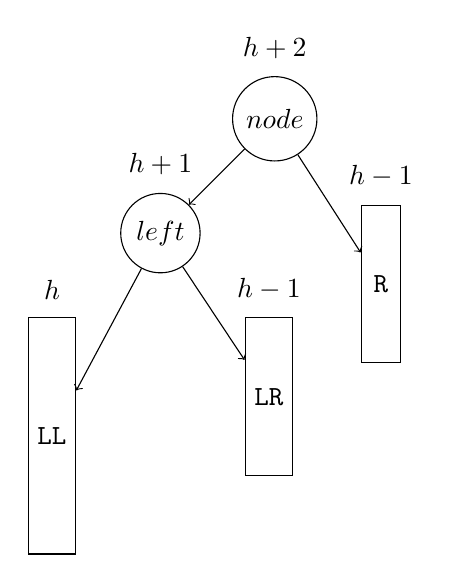
\begin{tikzpicture}
      \node[circle, draw] (node) at (1, 1) {$node$};
      \node[circle, draw] (left) [below left = 1cm of node] {$left$};
      \node[rectangle, minimum height = 2cm, minimum width = 0.5cm, draw] (subtreeR) [below right = 1cm of node] {\texttt{R}};
      \node[rectangle, minimum height = 3cm, minimum width = 0.5cm, draw] (subtreeLL) [below left = 1cm of left] {\texttt{LL}};
      \node[rectangle, minimum height = 2cm, minimum width = 0.5cm, draw] (subtreeLR) [below right = 1cm of left] {\texttt{LR}};

      % alturas
      \node [above = 0.1cm of node] {$h + 2$};
      \node [above = 0.1cm of left] {$h + 1$};
      \node [above = 0.1cm of subtreeLL] {$h$};
      \node [above = 0.1cm of subtreeLR] {$h - 1$};
      \node [above = 0.1cm of subtreeR] {$h - 1$};

      \draw (node) edge[->] (left);
      \draw (node) edge[->] (subtreeR);
      \draw (left) edge[->] (subtreeLL);
      \draw (left) edge[->] (subtreeLR);
    \end{tikzpicture}
  }
  \quad
  \subfigure[Depois da rotação]{
    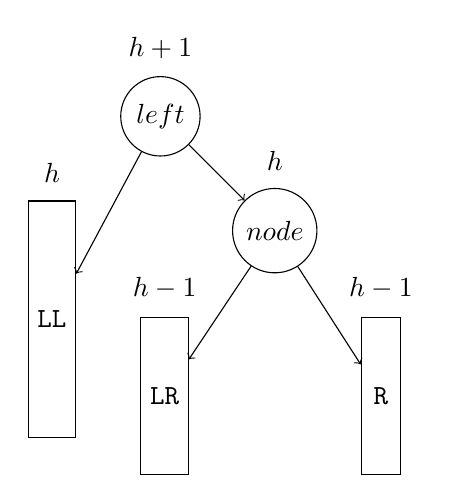
\begin{tikzpicture}
      \node[circle, draw] (left) at (1, 1) {$left$};
      \node[circle, draw] (node) [below right = 1cm of left] {$node$};
      \node[rectangle, minimum height = 3cm, minimum width = 0.5cm, draw] (subtreeLL) [below left = 1cm of left] {\texttt{LL}};
      \node[rectangle, minimum height = 2cm, minimum width = 0.5cm, draw] (subtreeLR) [below left = 1cm of node] {\texttt{LR}};
      \node[rectangle, minimum height = 2cm, minimum width = 0.5cm, draw] (subtreeR) [below right = 1cm of node] {\texttt{R}};


      % alturas
      \node [above = 0.1cm of node] {$h$};
      \node [above = 0.1cm of left] {$h + 1$};
      \node [above = 0.1cm of subtreeLL] {$h$};
      \node [above = 0.1cm of subtreeLR] {$h - 1$};
      \node [above = 0.1cm of subtreeR] {$h - 1$};

      \draw (left) edge[->] (node);
      \draw (node) edge[->] (subtreeR);
      \draw (left) edge[->] (subtreeLL);
      \draw (node) edge[->] (subtreeLR);
    \end{tikzpicture}
  }
  \caption{Rotação simples à direita.  Nós representados como círculos
    e sub-árvores como retângulos.  Acima dos nós e sub-árvores,
    representamos sua altura.}
\label{org1c4833f}
\end{figure}

Para resolver o caso 1, usamos uma rotação simples à direita.  A
Figura \ref{org1c4833f} ilustra o procedimento dessa rotação.  Note que
trata-se apenas da atualização do conteúdo de dois nós, e de
algumas atualizações de referências.  Assim, essa rotação pode ser
executada em tempo constante, e após feita, é necessário atualizar
as alturas de \(node\) e \(left\).

\begin{figure}[h]
  \centering
  \subfigure[Antes da rotação]{
    \scalebox{0.6}{
      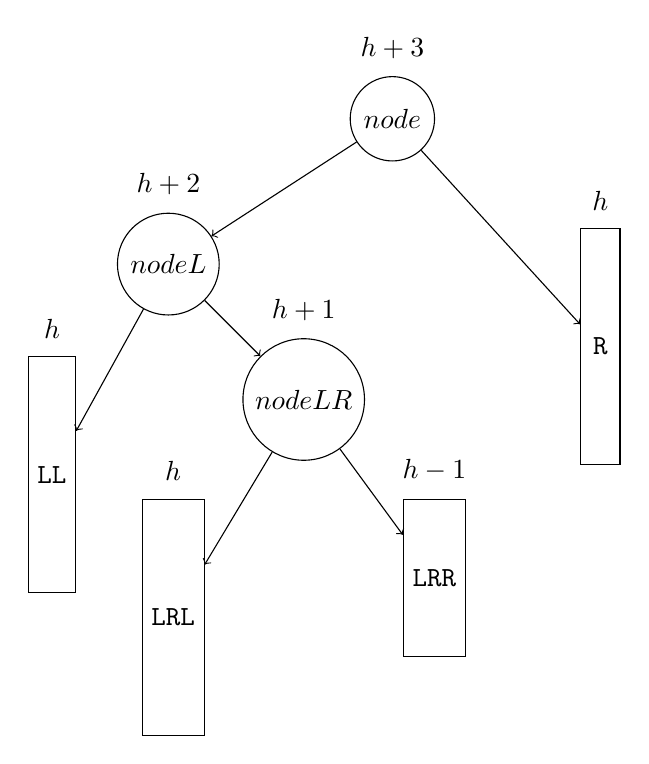
\begin{tikzpicture}
        \node[circle, draw] (node) at (1, 1) {$node$};
        \node[rectangle, minimum height = 3cm, minimum width = 0.5cm, draw] (subtreeR) [below right = 1cm and 2cm of node] {\texttt{R}};
        \node[circle, draw] (nodeL) [below left = 1cm and 2cm of node] {$nodeL$};
        \node[circle, draw] (nodeLR) [below right = 1cm of nodeL] {$nodeLR$};
        \node[rectangle, minimum height = 3cm, minimum width = 0.5cm, draw] (subtreeLL) [below left = 1cm of nodeL] {\texttt{LL}};
        \node[rectangle, minimum height = 3cm, minimum width = 0.5cm, draw] (subtreeLRL) [below left = 1cm of nodeLR] {\texttt{LRL}};
        \node[rectangle, minimum height = 2cm, minimum width = 0.5cm, draw] (subtreeLRR) [below right = 1cm of nodeLR] {\texttt{LRR}};

        \node [above = 0.1cm of subtreeLRL] {$h$};
        \node [above = 0.1cm of subtreeLRR] {$h - 1$};
        \node [above = 0.1cm of nodeLR] {$h + 1$};
        \node [above = 0.1cm of subtreeLL] {$h$};
        \node [above = 0.1cm of nodeL] {$h + 2$};
        \node [above = 0.1cm of subtreeR] {$h$};
        \node [above = 0.1cm of node] {$h + 3$};

        \draw (node) edge[->] (subtreeR);
        \draw (node) edge[->] (nodeL);
        \draw (nodeL) edge[->] (subtreeLL);
        \draw (nodeL) edge[->] (nodeLR);
        \draw (nodeLR) edge[->] (subtreeLRL);
        \draw (nodeLR) edge[->] (subtreeLRR);
      \end{tikzpicture}
    }
  }
  \subfigure[Depois da primeira rotação]{
    \scalebox{0.6}{
      \begin{tikzpicture}
        \node[circle, draw] (node) at (1, 1) {$node$};
        \node[rectangle, minimum height = 3cm, minimum width = 0.5cm, draw] (subtreeR) [below right = 1cm and 2cm of node] {\texttt{R}};
        \node[circle, draw] (nodeLR) [below left = 1cm of node] {$nodeLR$};
        \node[circle, draw] (nodeL) [below left = 1cm and 2cm of nodeLR] {$nodeL$};
        \node[rectangle, minimum height = 3cm, minimum width = 0.5cm, draw] (subtreeLL) [below left = 1cm of nodeL] {\texttt{LL}};
        \node[rectangle, minimum height = 3cm, minimum width = 0.5cm, draw] (subtreeLRL) [below right = 1cm of nodeL] {\texttt{LRL}};
        \node[rectangle, minimum height = 2cm, minimum width = 0.5cm, draw] (subtreeLRR) [below right = 1cm of nodeLR] {\texttt{LRR}};

        \node [above = 0.1cm of subtreeLL] {$h$};
        \node [above = 0.1cm of subtreeLRL] {$h$};
        \node [above = 0.1cm of nodeL] {$h + 1$};
        \node [above = 0.1cm of subtreeLRR] {$h - 1$};
        \node [above = 0.1cm of nodeLR] {$h + 2$};
        \node [above = 0.1cm of subtreeR] {$h$};
        \node [above = 0.1cm of node] {$h + 3$};

        \draw (node) edge[->] (subtreeR);
        \draw (node) edge[->] (nodeLR);
        \draw (nodeL) edge[->] (subtreeLL);
        \draw (nodeL) edge[->] (subtreeLRL);
        \draw (nodeLR) edge[->] (subtreeLRR);
        \draw (nodeLR) edge[->] (nodeL);
      \end{tikzpicture}
    }
  }
  \subfigure[Depois da segunda rotação]{
    \scalebox{0.6}{
      \begin{tikzpicture}
        \node[circle, draw] (nodeLR) at (1, 1) {$nodeLR$};
        \node[circle, draw] (nodeL) [below left = 1cm and 2cm of nodeLR] {$nodeL$};
        \node[circle, draw] (node) [below right = 1cm and 2cm of nodeLR] {$node$};
        \node[rectangle, minimum height = 3cm, minimum width = 0.5cm, draw] (subtreeLL) [below left = 1cm of nodeL] {\texttt{LL}};
        \node[rectangle, minimum height = 3cm, minimum width = 0.5cm, draw] (subtreeLRL) [below right = 1cm of nodeL] {\texttt{LRL}};
        \node[rectangle, minimum height = 3cm, minimum width = 0.5cm, draw] (subtreeR) [below right = 1cm and 2cm of node] {\texttt{R}};
        \node[rectangle, minimum height = 2cm, minimum width = 0.5cm, draw] (subtreeLRR) [below left = 1cm of node] {\texttt{LRR}};

        \node [above = 0.1cm of subtreeLL] {$h$};
        \node [above = 0.1cm of subtreeLRL] {$h$};
        \node [above = 0.1cm of subtreeLRR] {$h - 1$};
        \node [above = 0.1cm of subtreeR] {$h$};
        \node [above = 0.1cm of nodeL] {$h + 1$};
        \node [above = 0.1cm of node] {$h + 1$};
        \node [above = 0.1cm of nodeLR] {$h + 2$};

        \draw (nodeLR) edge[->] (node);
        \draw (nodeLR) edge[->] (nodeL);
        \draw (nodeL) edge[->] (subtreeLL);
        \draw (nodeL) edge[->] (subtreeLRL);
        \draw (node) edge[->] (subtreeR);
        \draw (node) edge[->] (subtreeLRR);
      \end{tikzpicture}
    }
  }
  \caption{Rotação dupla: à esquerda em um nível mais baixo, e à
    direita em um nível mais alto.  Nós são círculos e sub-árvores são
    retângulos. Acima de cada nó e sub-árvore está representada sua altura.}
\label{orga3bbf5d}
\end{figure}

No caso 2, é necessário fazer uma rotação dupla.  A Figura
\ref{orga3bbf5d} traz uma ilustração de como tal rotação é feita.
Primeiro, faz-se uma rotação simples à esquerda no filho esquerdo,
e em seguida uma rotação simples à direita no nó.  Novamente, essa
rotação tem um custo constante, e quando realizada, devem ser
atualizadas as alturas de \(node\), \(nodeL\) e \(nodeLR\).  Como os
casos \emph{right-heavy} são meros ``espelhos'' dos casos aqui
ilustrados, rotações análogas às apresentadas são suficientes para
corrigí-los.

\begin{exercicio}
Descreva uma forma de converter uma Árvore Binária de Busca com
\(n\) nós em uma Árvore AVL em tempo \(O(n \log n)\).
\end{exercicio}

\begin{exercicio}
Em uma árvore binária, um nó é dito filho único sse ele tem pai e
seu nó pai tem exatamente um filho.  Vamos definir a \emph{razão de
solidão} de uma árvore binária \(T\) (\(RS(T)\)) como o número de
filhos únicos em \(T\) dividido pelo número de nós de \(T\).  Prove
que, se \(T\) é uma Árvore AVL, então \(RS(T) \leq \frac{1}{2}\).
Dica: quais nós de uma Árvore AVL podem ser filhos únicos?
\end{exercicio}

\clearpage

\subsubsection{Implementação}
\label{sec:org6ff4c56}

Vamos mostrar uma abordagem de implementação de Árvores AVL
utilizando herança a partir de \texttt{BSTree}.  Para isso, o código de
\texttt{BSTree} precisou sofrer alguma refatoração, e assim permitir um
maior reuso de seus métodos.  Vamos explicar a refatoração
realizada sempre que for necessário.

\begin{minted}[,fontsize=\footnotesize]{c++}
#pragma once
// for max function
#include <algorithm>
// smart pointers
#include <memory>
// optional type
#include <optional>
// stack type
#include <stack>
// we are going to inherit from BSTree
#include <bstree.hpp>
\end{minted}

Não há muita novidade nos cabeçalhos.  Importamos \texttt{algorithm} para
usar a função \texttt{std::max} e \texttt{stack} para utilizar pilhas como uma
representação de caminhos da raiz até um certo nó da árvore.  Além
disso, utilizaremos \texttt{bstree.hpp} para fazer a herança.

\begin{minted}[,fontsize=\footnotesize]{c++}
template<typename Key, typename Val>
class AVLTree : public BSTree<Key, Val>{
  // ...
}
\end{minted}

Descrevemos a classe \texttt{AVLTree} como uma subclasse de \texttt{BSTree}, sob
os mesmos parâmetros de chave e valor.  É certo que não faria
muito sentido, por exemplo, que \texttt{AVLTree<int, char>} fosse
subclasse de \texttt{BSTree<std::string, int>}.  Vamos descrever os
membros de \texttt{AVLTree}.

\pagebreak

\begin{minted}[,fontsize=\footnotesize]{c++}
private:
  // type alias for saving us from some typing
  using BST = BSTree<Key, Val>;
  // the node of AVLTree
  struct AVLTreeNode{
    // ...
  };
  // returns heights of left and right subtrees
  static std::pair<int, int> childrenHeights(const AVLTreeNode* node){
    // ...
  }
  // calculates balance factor of a given node
  static int balanceFactor(const AVLTreeNode* node){
    // ...
  }
  // updates height of node based on the heights of its children
  static void updateHeight(AVLTreeNode* node){
    // ...
  }
  // ...
\end{minted}

Começando a descrição dos membros privados de \texttt{AVLTree}, temos uma
\texttt{struct} para representar o nó de uma \texttt{AVLTree}, \texttt{AVLTreeNode}.
Vale lembrar que, com a refatoração, também transformamos
\texttt{BSTreeNode} em uma \texttt{struct}, e minimizamos a quantidade de
operações delegadas aos nós.  Agora, apenas delegamos \texttt{minKey} e
\texttt{maxKey}.

Em \texttt{C++}, não há muita diferença entre \texttt{struct} e \texttt{class}. A única
distinção é que, por padrão, membros de \texttt{struct} são públicos e
membros de \texttt{class} são privados.  No entanto, é boa prática
designar como \texttt{struct} entidades mais simples (como os nós, que
passaram a ser após a refatoração) e como \texttt{class} entidades mais
complexas.

Mantendo a simplicidade de \texttt{AVLTreeNode}, três funções auxiliares
são implementadas como \texttt{static}, e não como métodos de
\texttt{AVLTreeNode}.  A função \texttt{childrenHeights} retorna um par de
\texttt{int}, cada um sendo a altura de um filho.  A função
\texttt{balanceFactor} retorna o \(balance\) de um nó passado como
argumento.  Por fim, a função \texttt{updateHeight} atualiza a altura de
um nó, baseando-se apenas na altura de seus filhos.  Vamos
descrever em detalhes \texttt{AVLTreeNode}.

\pagebreak

\begin{minted}[,fontsize=\footnotesize]{c++}
struct AVLTreeNode{
  Key key;
  Val val;
  // smart pointers
  std::unique_ptr<AVLTreeNode> left;
  std::unique_ptr<AVLTreeNode> right;
  // height of node (no negative value makes sense)
  unsigned int height;
  // initializes AVLTreeNode.  Since it has no children, it has
  // height zero
  AVLTreeNode(Key k, Val v) : key{k},
                              val{v},
                              left{nullptr},
                              right{nullptr},
                              height{0}
  {}
  // returns Key Val pair whose Key is maximum.  We need this
  // information on every subtree for the removal algorithm
  std::pair<Key, Val> maxKey() const {
    // ...
  }
  // returns Key Val pair whose Key is minimum
  std::pair<Key, Val> minKey() const {
    // ...
  }
};
\end{minted}

Em \texttt{AVLTreeNode}, temos os mesmos campos de \texttt{BSTreeNode}, mais um
inteiro não-negativo para representar a altura do nó.  Os métodos
\texttt{minKey} e \texttt{maxKey} têm a mesma implementação de \texttt{BSTreeNode}, e
portanto não precisam ser apresentados.  Inclusive, esse é o único
reuso que não faremos.

O motivo por trás da refatoração são os ponteiros \texttt{left} e
\texttt{right}.  Note que, em \texttt{BSTreeNode}, eles apontam para tipos
diferentes de nós, e portanto não poderíamos utilizá-los em
\texttt{AVLTreeNode} caso \texttt{AVLTreeNode} fosse subclasse de \texttt{BSTreeNode}
(até poderíamos, mas eu não gosto de fazer \emph{casting}).  Como não
podemos ter herança entre os nós, boa parte do código de
\texttt{BSTreeNode} foi passado para \texttt{BSTree}, a fim de maximizar o
reuso.  Os métodos \texttt{minKey} e \texttt{maxKey} permanecem nos nós porque
precisamos dessa informação, em cada sub-árvore, para o
procedimento de remoção.

\pagebreak

\begin{minted}[,fontsize=\footnotesize]{c++}
// returns heights of left and right subtrees
static std::pair<int, int> childrenHeights(const AVLTreeNode* node){
  // get height of left and right subtrees
  int leftHeight  = node->left  ? node->left->height  : -1;
  int rightHeight = node->right ? node->right->height : -1;

  return std::make_pair(leftHeight, rightHeight);
}
\end{minted}

A implementação de \texttt{childrenHeights} é conforme a definição de
altura, inclusive quanto à convenção adotada para sub-árvores
vazias.  Como \texttt{childrenHeights} não deve alterar seu argumento,
ele é recebido como \texttt{const}.  Perceba ainda que, apesar da altura
de um nó ser \texttt{unsigned int}, a altura de uma sub-árvore vazia
precisa ser \texttt{int}.

\begin{minted}[,fontsize=\footnotesize]{c++}
// calculates balance factor of a given node
static int balanceFactor(const AVLTreeNode* node){
  auto[leftHeight, rightHeight] = childrenHeights(node);

  return rightHeight - leftHeight;
}
\end{minted}

A função \texttt{balanceFactor} não exige grandes explicações.  Vale
notar, de qualquer maneira, que seu argumento é recebido como
\texttt{const}.

\begin{minted}[,fontsize=\footnotesize]{c++}
// updates height of node based on the heights of its children
static void updateHeight(AVLTreeNode* node){
  // get height of left and right subtrees
  auto[leftHeight, rightHeight] = childrenHeights(node);
  // calculates new height
  unsigned int newHeight = std::max(leftHeight, rightHeight) + 1;
  node->height = newHeight;
}
\end{minted}

A implementação de \texttt{updateHeight} é bastante intuitiva.  Note o
uso de \texttt{std::max} para calcular a maior altura entre os filhos de
\texttt{node}.

\begin{minted}[,fontsize=\footnotesize]{c++}
private:
  // ...
  // implementation of AVLTree
  template<typename Node>
  class AVLTreeWithNode : public BST::template BSTreeWithNode<Node>{
    // ...
  };
\end{minted}

Uma parte importante da refatoração é que a implementação de
\texttt{BSTree} passou para a nova classe \texttt{BSTreeWithNode}.  Em
\texttt{BSTreeWithNode}, o tipo de nó a ser utilizado é recebido como um
parâmetro.  Dessa forma, \texttt{AVLTreeWithNode} pode ser subclasse de
\texttt{BSTreeWithNode} utilizando como nó \texttt{AVLTreeNode}.  No caso, quando
formos criar uma instância de \texttt{AVLTreeWithNode}, usaremos
\texttt{AVLTreeWithNode<AVLTreeNode>}, e isso fará com que o código de
\texttt{BSTreeWithNode} seja definido para \texttt{AVLTreeNode}.  Para
instanciar \texttt{BSTreeWithNode}, basta \texttt{BSTreeWithNode<BSTreeNode>}.

\begin{minted}[,fontsize=\footnotesize]{c++}
private:
  // ...
  template<typename Node>
  class AVLTreeWithNode : public BST::template BSTreeWithNode<Node>{
  private:
    // since BST is not instantiated yet, we need to tell the compiler
    // that BSTreeWithNode is a template and a type name when instantiated
    using BSTWithNode = typename BST::template BSTreeWithNode<Node>;
  public:
    // builds an empty AVLTree. Basically delegates all the work to BSTreeWithNode
    AVLTreeWithNode() : BSTWithNode{}
    {}
    // Creates an AVLTree with a nonempty root
    AVLTreeWithNode(Key key, Val val) : BSTWithNode{key, val}
    {}
    // inserts a Key Val pair in case Key is not present.  Return
    // indicates whether insertion occurred
    bool insert(Key key, Val val){
      // ...
    }
    // removes key in case it is present.  Return value indicates
    // whether removal has occurred
    bool remove(Key key){
      // ...
    }
  };
  // ...
\end{minted}

Com a descrição de \texttt{AVLTreeWithNode}, notamos que há o
aproveitamento completo dos métodos \texttt{isEmpty}, \texttt{sesrch}, \texttt{maxKey}
e \texttt{minKey} de \texttt{BSTreeWithNode}.  Os métodos que modificam a
estrutura, \texttt{insert} e \texttt{remove}, farão um reuso parcial das
funcionalidades correspondentes de \texttt{BSTreeWithNode}.  Isso se deve
ao fato de que, após fazerem sua operação usual, eles precisam
manter a invariante de balanceamento de \texttt{AVLTreeWithNode}.  Vamos
descrever protótipos desses métodos (que deverão ser completado em
laboratório).

\pagebreak

\begin{minted}[,fontsize=\footnotesize]{c++}
// inserts a Key Val pair in case Key is not present.  Return
// indicates whether insertion occurred
bool insert(Key key, Val val){
  // the actual insertion is made by BSTReeWithNode
  bool hasInserted = BSTWithNode::insert(key, val);
  // if insertion really happened ...
  if (hasInserted){
    // ... do avl stuff
  }

  return hasInserted;
}
\end{minted}

Como podemos ver, o método \texttt{insert} delega a operação de inserção
para \texttt{BSTreeWithNode}.  Caso a inserção tenha de fato ocorrido,
então é necessário verificar e manter o balanceamento de
\texttt{AVLTreeWithNode}.  Essa parte deve ser escrita em laboratório.

\begin{minted}[,fontsize=\footnotesize]{c++}
// removes key in case it is present.  Return value indicates
// whether removal has occurred
bool remove(Key key){
  // first we verify if key is present
  bool hasKey = BSTWithNode::search(key);
  // in case it is, removal will occurr
  if (hasKey){
    // performs removal, and returns parent key in case root was not deleted
    std::optional<Key> parentKey = BSTWithNode::removeExistingKey(key);
    // in case a node other than root has been deleted ...
    if (parentKey){
      // ... do avl stuff
    }
    return true;
  }
  // otherwise, we simply indicate that removal has not occurred
  else{
    return false;
  }
}
\end{minted}

O método \texttt{remove} apresenta mais um produto da refatoração de
\texttt{BSTree}, que é o método \texttt{protected} \texttt{removeExistingKey}.  A
finalidade de \texttt{removeExistingKey} é encapsular toda a lógica de
remoção de uma chave existente na árvore, e deixar para o \texttt{remove}
de \texttt{BSTreeWithNode} apenas o trabalho de verificar se a chave a
ser removido existe e, em caso afirmativo, chamar
\texttt{removeExistingKey}.  A ideia por trás disso é que \texttt{remove}
continua retornando \texttt{bool}, que é significativo para o usuário,
mas \texttt{removeExistingKey} retorna um \texttt{optional} contendo a chave do
pai do nó que foi deletado (caso ele tenha um pai, daí o
\texttt{optional}).  Dessa forma, o retorno de \texttt{removeExistingKey}
facilita a implementação de \texttt{AVLTreeWithNode}.

Em sua lógica, \texttt{remove} se assemelha a \texttt{insert}.  É verificada a
existência da chave a ser removida.  Caso ela esteja presente na
árvore, a remoção é delegada para \texttt{BSTreeWithNode}.  Com a
informação fornecida por \texttt{removeExistingKey}, é possível manter o
balanceamento de \texttt{AVLTreeWithNode}, caso seja necessário.  Essa
parte da implementação deve ser feita em laboratório.

Para facilitar a implementação do balanceamento de
\texttt{AVLTreeWithNode}, existem alguns métodos \texttt{static} que auxiliam
certas tarefas.  Vamos descrevê-los a seguir.

\begin{minted}[,fontsize=\footnotesize]{c++}
// rebalances a node
static void rebalanceNode(AVLTreeNode* node){
  // calculates balance factor
  int nodeBalanceFactor = balanceFactor(node);
  // node is left-heavy
  if (nodeBalanceFactor <= -2){
    int leftBalanceFactor = balanceFactor(node->left.get());
    if (leftBalanceFactor <= -1){
      // which rotation?
    }
    else{
      // which rotation?
    }
  }
  // node is right-heavy
  else if (nodeBalanceFactor >= 2){
    int rightBalanceFactor = balanceFactor(node->right.get());
    if (rightBalanceFactor >= 1){
      // which rotation?
    }
    else{
      // which rotation?
    }
  }
}
\end{minted}

O método estático \texttt{rebalanceNode} utiliza \texttt{balanceFactor} para
determinar a lógica de balanceamento, e assim decidir qual rotação
deve ser aplicada.  Vamos descrever uma rotação simples à direita,
para ilustrar como deve ser realizado esse tipo de operação.

\pagebreak

\begin{minted}[,fontsize=\footnotesize]{c++}
// performs a simple right rotation on node
static void rotateR(AVLTreeNode* node){
  // first we set aside all the moving subtrees
  std::unique_ptr<AVLTreeNode> subtreeLL = std::move(node->left->left);
  std::unique_ptr<AVLTreeNode> subtreeLR = std::move(node->left->right);
  std::unique_ptr<AVLTreeNode> subtreeR  = std::move(node->right);
  // then we save the contents of the moving nodes
  std::pair<Key, Val> nodeContent      = std::make_pair(node->key, node->val);
  std::pair<Key, Val> leftChildContent = std::make_pair(node->left->key, node->left->val);
  // left child becomes node
  node->key = leftChildContent.first;
  node->val = leftChildContent.second;
  // node becomes the right child
  node->right = std::make_unique<AVLTreeNode>(nodeContent.first, nodeContent.second);
  // finally we rearrange the moving subtrees ...
  node->left         = std::move(subtreeLL);
  node->right->left  = std::move(subtreeLR);
  node->right->right = std::move(subtreeR);
  // ... and update heights on the affected nodes
  updateHeight(node->right.get());
  updateHeight(node);
}
\end{minted}

Os comentários de \texttt{rotateR} descrevem bem seu funcionamento.  É
deixado como exercício prático implementar as demais rotações.

Para manter o balanceamento de \texttt{AVLTreeWithNode}, é necessário
atualizar a altura de cada nó no caminho afetado pela modificação,
``de baixo para cima''.  Após isso, percorre-se o mesmo caminho de
nós, na mesma direção, efetuando os rebalanceamentos.  A função
\texttt{pathToExistingKey} de \texttt{BSTreeWithNode}, se usada adequadamente,
nos permite determinar tal caminho a ser corrigido,
representando-o como uma pilha de \texttt{AVLTreeNode*}.

\begin{minted}[,fontsize=\footnotesize]{c++}
// the compiler will deduce what Function is.  Applies func to each
// node on path
template<typename Function>
static void applyOnPath(Function func, std::stack<AVLTreeNode*> path){
  // node to have function applied on
  AVLTreeNode* currentNode = nullptr;
  // while there are nodes to be visited
  while (!path.empty()){
    // gets a new node
    currentNode = path.top();
    // apply function
    func(currentNode);
    // then discards its reference
    path.pop();
  }
}
\end{minted}

A função \texttt{applyOnPath} executa uma operação em todas as
referências de nó armazenadas numa pilha, em sua ordem de remoção.
Essa é a base lógica tanto para atualizarmos as alturas de nós em
um caminho afetado por modificações, quanto para realizarmos os
devidos balanceamentos nos mesmos nós.  As funções responsáveis
por essas duas tarefas são descritas a seguir.

\begin{minted}[,fontsize=\footnotesize]{c++}
// does the necessary height updates for nodes on path
static void updateHeightsOnPath(std::stack<AVLTreeNode*> path){
  // notice how we do not need to specify Function
  applyOnPath(updateHeight, path);
}
// rebalances each node on path
static void rebalanceNodesOnPath(std::stack<AVLTreeNode*> path){
  applyOnPath(rebalanceNode, path);
}
\end{minted}

Essencialmente, cada uma dessas funções é uma aplicação de
\texttt{applyOnPath} com uma função diferente.  Esse tipo de função, que
recebe outras funções como argumentos, é chamado de \emph{função de alta
ordem}.

\begin{minted}[,fontsize=\footnotesize]{c++}
private:
  // ...
  // AVLTree with proper node type
  AVLTreeWithNode<AVLTreeNode> avlt;
// ...
\end{minted}

Por fim, temos o último membro privado de \texttt{AVLTree}, que é
justamente uma instância de \texttt{AVLTreeWithNode} utilizando
\texttt{AVLTreeNode} como seu tipo de nó.  Dessa forma, os métodos
públicos de \texttt{AVLTree} apenas precisam ser redirecionados para os
métodos públicos de \texttt{avlt}.

\pagebreak

\begin{minted}[,fontsize=\footnotesize]{c++}
public:
  // builds an empty AVLTree
  AVLTree() : avlt{}
  {}
  // Creates an AVLTree with a nonempty root
  AVLTree(Key key, Val val) : avlt{key, val}
  {}
  // inserts a Key Val pair in case Key is not present.  Return
  // indicates whether insertion occurred
  bool insert(Key key, Val val){
    return avlt.insert(key, val);
  }
  // removes key in case it is present.  Return value indicates
  // whether removal has occurred
  bool remove(Key key){
    return avlt.remove(key);
  }
  // returns Val attached to Key.  In case Key is not present, returns
  // nothing
  std::optional<Val> search(Key key) const {
    return avlt.search(key);
  }
  // returns Key Val pair whose Val corresponds to the maximum BSTree
  // Key.  In case tree is empty, returns nothing
  std::optional<std::pair<Key, Val>> maxKey() const {
    return avlt.maxKey();
  }
  // returns Key Val pair whose Val corresponds to the minimum BSTree
  // Key.  In case tree is empty, returns nothing
  std::optional<std::pair<Key, Val>> ninKey() const {
    return avlt.ninKey();
  }
\end{minted}

\subsubsection{Análise de Complexidade}
\label{sec:orgda25ea9}

Como sabemos, uma Árvore Binária de Busca com altura \(h\) tem as
suas operações com custo \(O(h)\).  Uma Árvore Binária de Busca com
\(n\) nós tem, no melhor caso, \(h \in O(\log n)\) e, no pior caso, \(h
    \in O(n)\).

Em uma Árvore AVL com \(n\) nós, o custo das operações é o mesmo de
uma Árvore Binária de Busca de altura \(O(\log n)\), acrescido do
custo de manutenção do balanceamento.  Como atualização de altura
e rotações são operações de tempo constante, e uma Árvore AVL
precisa realizar cada uma dessas operações em um caminho de nós
até a raiz, esse custo adicional é \(O(\log n)\), já que sua altura
é \(O(\log n)\).  Assim, o custo total das operações de uma Árvore
AVL é \(O(\log n)\).

\subsection{Árvores Rubro-Negras}
\label{sec:orgef19a56}

Continuando com o tópico de estruturas de dados autoajustáveis,
apresentamos mais um tipo de Árvore Binária de Busca com uma boa
altura.  Dessa vez, usaremos um critério diferente para determinar
um bom balanceamento.

\subsubsection{Definição}
\label{sec:org3e3eb67}

Uma Árvore Rubro-Negra é uma Árvore Binária de Busca cujos nós,
além das informações usuais, trazem consigo um atributo de cor que
pode assumir exatamente um de dois valores: ou vermelho ou preto.
Com esse novo atributo, Árvores Rubro-Negras conseguem estabelecer
a propriedade de que nenhum caminho da raiz a uma folha tem o
dobro de nós de outro tal caminho, o que garante um balanceamento
razoável, certamente não tão bom quanto o de uma Árvore AVL.

As seguintes propriedades devem ser satisfeitas por uma Árovre
Rubro-Negra:
\begin{enumerate}
\item \label{org01575c0} Sua raiz é um nó preto;
\item Toda folha é um nó preto;
\item \label{org64120cd} Se um nó é vermelho, então seus filhos
são nós pretos;
\item \label{org76cf2e3} Para cada nó, todos os caminhos a
partir dele até uma folha contêm o mesmo número de nós pretos.
\end{enumerate}

Vamos convencionar que, em vez de sub-árvores vazias, nós podem
ter folhas pretas que não contém dados significativos.  Dessa
forma, todo nó significativo da árvore é um nó interno, e
trataremos o tamanho de uma Árvore Rubro-Negra pelo número de seus
nós internos (nós que não são folhas).

\begin{exercicio}
Prove que um nó vermelho tem exatamente dois filhos.
\end{exercicio}

\begin{exercicio}
Prove que um nó vermelho não pode ter seu pai com cor vermelha.
\end{exercicio}

Definimos \(bh(node)\) (onde \(bh\) denota \emph{black height}) como o
número de nós pretos em um caminho qualquer a partir de \(node\)
(mas sem incluir \(node\)) até uma folha.  A propriedade
\ref{org76cf2e3} garante que \(bh\) está bem definido para
qualquer nó.

\begin{theorem}
\label{org96b101c}
Uma Árvore Rubro-Negra com \(n\) nós internos tem altura no máximo
\(2\log (n + 1)\).
\end{theorem}

\begin{proof}
Inicialmente, vamos mostrar que a sub-árvore enraizada em \(node\)
contém no mínimo \(2^{bh(node)} - 1\) nós internos.  Vamos provar
isso por indução na altura de \(node\).  Se \(node\) tem altura \(0\),
então \(node\) é uma folha e portanto sua sub-árvore tem \(0\) nós
internos, o que está de acordo com o mínimo de \(2^{hb(node)} - 1 =
    2^0 - 1 = 0\) nós internos.  Agora tome \(node\) com altura positiva.
Dessa forma, \(node\) é um nó interno e, conforme a nossa convenção,
\(node\) tem dois filhos.  Cada filho de \(node\) tem seu \(bh\) igual a
ou \(bh(node)\) (quando o filho é vermelho) ou \(bh(node) - 1\)
(quando o filho é preto).  Com isso, sabemos que o \(bh\) de um
filho de \(node\) é pelo menos \(bh(node) - 1\).  Como os filhos de
\(node\) têm altura menor que a de \(node\), podemos concluir, por
hipótese, que a sub-árvore de cada filho de \(node\) tem no mínimo
\(2^{bh(node) - 1} - 1\) nós internos.  Com isso, a sub-árvore de
\(node\) contém ao menos \(2(2^{bh(node) - 1} - 1) + 1 =
    2^{bh(node)} - 2 + 1 = 2^{bh(node)} - 1\) nós internos.

Seja \(h\) a altura da árvore.  De acordo com a propriedade
\ref{org64120cd}, um caminho a partir da raiz até uma folha
(mas sem incluir a raiz) tem no mínimo metade de seus nós pretos
(Exercício \ref{orgf2a1ed6}), o que implica que o \(bh\) da
raiz é no mínimo \(\frac{h}{2}\).  Como a árvore tem \(n\) nós
internos, sabemos que
\begin{align}
n \geq            &\, 2^{\frac{h}{2}} - 1 \\
n + 1 \geq        &\, 2^{\frac{h}{2}} \\
\log (n + 1) \geq &\, \log (2^{\frac{h}{2}}) \\
\log (n + 1) \geq &\, \frac{h}{2} \\
h \leq            &\, 2\log (n + 1)
\end{align}
\end{proof}

\begin{exercicio}
\label{orgf2a1ed6}
Prove que um caminho a partir da raiz até uma folha (mas sem
incluir a raiz) tem no mínimo metade de seus nós pretos.
\end{exercicio}

Como consequência do Teorema \ref{org96b101c}, sabemos que as
operações em uma Árvore Rubro-Negra tem custo \(O(\log n)\).  No
entanto, é preciso assegurar que as operações modificadoras
(inserção e remoção) mantenham as propriedades esperadas de uma
Árvore Rubro-Negra.

\begin{exercicio}
Prove que, em qualquer sub-árvore de uma Árvore Rubro-Negra, o
caminho mais longo de sua raiz a uma folha tem no máximo o dobro
do número de nós do caminho mais curto de sua raiz até uma folha.
\end{exercicio}

\subsubsection{Manutenção}
\label{sec:org0fc343d}

Diferente de Árvores AVL, Árvores Rubro-Negras precisam apenas de
rotações simples para a manutenção de suas propriedades.  No
entanto, pode ser preciso também modificar a cor de certos nós.
Dessa forma, como rotações simples já foram ilustradas na Subseção
\ref{org6ea5e87}, vamos discutir principalmente as mudanças de cor
necessárias para as operações de inserção e remoção.

A operação de inserção é realizada da mesma forma que em uma
Árvore Binária de Busca, e insere o novo nó (que chamaremos de
\(node\)) como um nó interno, pai de duas folhas pretas.  Para não
perturbar a propriedade \ref{org76cf2e3}, \(node\) deve ter
cor vermelha.  Porém, é possível que \(node\) tenha pai, e esse
(\(parentNode\)) também seja vermelho, o que violaria a propriedade
\ref{org64120cd}.  Caso \(node\) não tenha pai, \(node\) é a raiz
e estamos violando a propriedade \ref{org01575c0}.

Se \(node\) for a raiz, podemos colorir \(node\) de preto sem prejuízo
para as propriedades.  No caso de \(node\) não ser raiz, vamos olhar
para seu tio (\(uncleNode\), irmão de \(parentNode\)) em três casos,
e em cada um deles vamos fazer \(node\) respeitar a propriedade
\ref{org64120cd} sem violar as demais:
\begin{enumerate}
\item \label{org84095da} \(uncleNode\) é vermelho: como \(parentNode\) é
vermelho e respeitava as propriedades antes da inserção de
\(node\), \(parentNode\) não é raiz e seu pai (\(grandParentNode\)) é
preto; assim, podemos ``descer'' a cor preta de
\(grandParentNode\), colorindo-o de vermelho e tornando pretos
seus filhos, \(parentNode\) e \(uncleNode\); isso corrige \(node\),
mas agora é preciso fazer a manutenção de \(grandParentNode\);
ilustramos esse procedimento na Figura \ref{orgf2fa004}.
\item \(uncleNode\) é preto e \(node\) é filho direito: aplicamos uma
rotação simples à esquerda em \(parentNode\), fazendo com que
\(parentNode\) torne-se filho esquerdo de \(node\), e portanto
precisamos fazer a manutenção de \(parentNode\), o que nos leva
ao caso \ref{orgb6f7dfa}; note que isso não viola a
propriedade \ref{org76cf2e3}, já que os dois nós
movidos são ambos vermelhos; a Figura \ref{org754ae44}
ilustra esse caso.
\item \label{orgb6f7dfa} \(uncleNode\) é preto e \(node\) é
filho esquerdo: assim como argumentado no caso \ref{org84095da},
\(grandParentNode\) existe e é preto; ``descemos'' a cor preta de
\(grandParentNode\) para \(parentNode\), o que pode violar a
propriedade \ref{org76cf2e3} para nós acima de
\(grandParentNode\) ou a propriedade \ref{org01575c0}, caso
\(grandParentNode\) seja raiz; para mitigar isso, aplicamos uma
rotação simples à direita em \(grandParentNode\); note que, como
\(grandParentNode\) (vermelho) passa a ser filho direito de
\(parentNode\) (preto), não há mais violações da propriedade
\ref{org64120cd}, e portanto nenhum nó que precise de
manutenção; a Figura \ref{org52743c4} sintetiza essa
operação.

\begin{figure}
  \centering
  \subfigure[Antes da operação]{
    \scalebox{0.7}{
      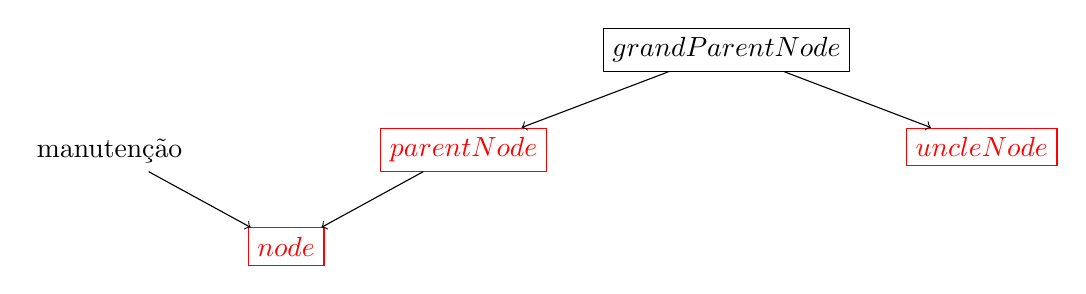
\begin{tikzpicture}
        \node[rectangle, draw, color = black] (gpNode) at (1, 1) {$grandParentNode$};
        \node[rectangle, draw, color = red] (pNode) [below left = 1cm of gpNode] {$parentNode$};
        \node[rectangle, draw, color = red] (uNode) [below right = 1cm of gpNode] {$uncleNode$};
        \node[rectangle, draw, color = red] (node) [below left = 1cm of pNode] {$node$};

        \node (m) [above left = 1cm of node] {manutenção};

        \draw (gpNode) edge[->] (pNode);
        \draw (gpNode) edge[->] (uNode);
        \draw (pNode) edge[->] (node);
        \draw (m) edge[->] (node);
      \end{tikzpicture}
    }
  }
  \subfigure[Depois da operação]{
    \scalebox{0.7}{
      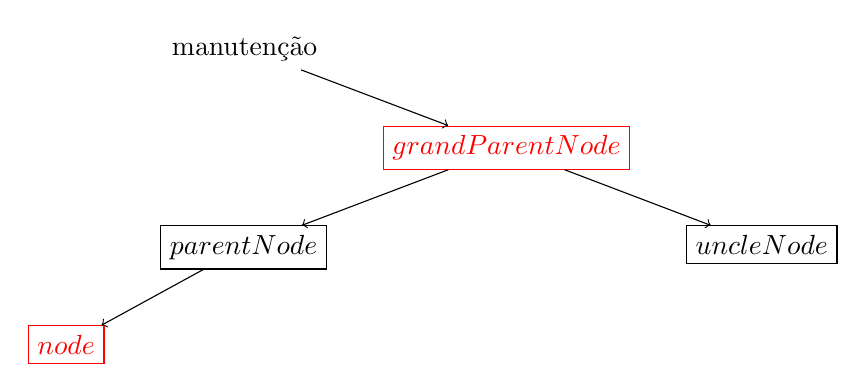
\begin{tikzpicture}
        \node[rectangle, draw, color = red] (gpNode) at (1, 1) {$grandParentNode$};
        \node[rectangle, draw, color = black] (pNode) [below left = 1cm of gpNode] {$parentNode$};
        \node[rectangle, draw, color = black] (uNode) [below right = 1cm of gpNode] {$uncleNode$};
        \node[rectangle, draw, color = red] (node) [below left = 1cm of pNode] {$node$};

        \node (m) [above left = 1cm of gpNode] {manutenção};

        \draw (gpNode) edge[->] (pNode);
        \draw (gpNode) edge[->] (uNode);
        \draw (pNode) edge[->] (node);
        \draw (m) edge[->] (gpNode);
      \end{tikzpicture}
    }
  }
  \caption{Ilustração do caso 1 da inserção.}
\label{orgf2fa004}
\end{figure}

\begin{figure}
  \centering
  \subfigure[Antes da operação]{
    \scalebox{0.7}{
      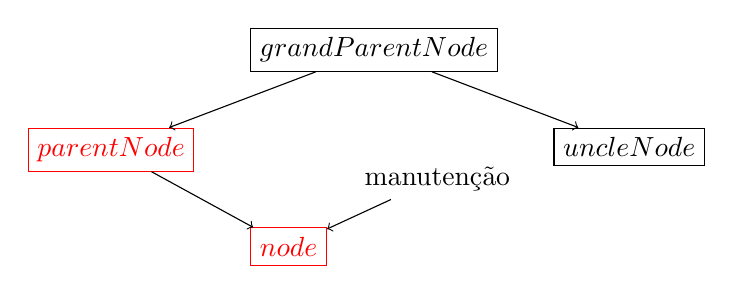
\begin{tikzpicture}
        \node[rectangle, draw, color = black] (gpNode) at (1, 1) {$grandParentNode$};
        \node[rectangle, draw, color = red] (pNode) [below left = 1cm of gpNode] {$parentNode$};
        \node[rectangle, draw, color = black] (uNode) [below right = 1cm of gpNode] {$uncleNode$};
        \node[rectangle, draw, color = red] (node) [below right = 1cm of pNode] {$node$};

        \node (m) [above right = 0.5cm of node] {manutenção};

        \draw (gpNode) edge[->] (pNode);
        \draw (gpNode) edge[->] (uNode);
        \draw (pNode) edge[->] (node);
        \draw (m) edge[->] (node);
      \end{tikzpicture}
    }
  }
  \subfigure[Depois da operação]{
    \scalebox{0.7}{
      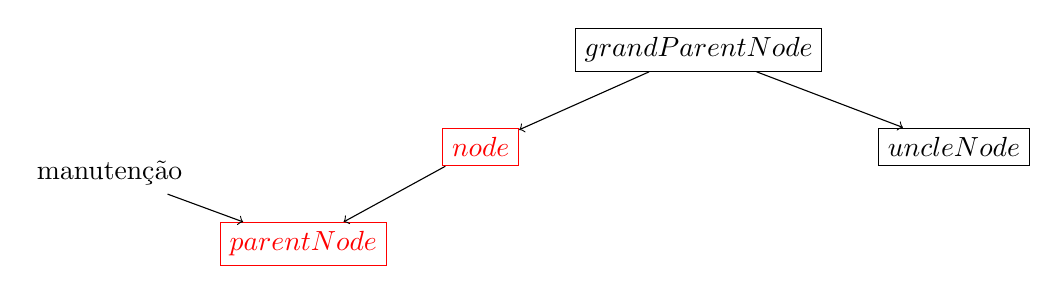
\begin{tikzpicture}
        \node[rectangle, draw, color = black] (gpNode) at (1, 1) {$grandParentNode$};
        \node[rectangle, draw, color = black] (uNode) [below right = 1cm of gpNode] {$uncleNode$};
        \node[rectangle, draw, color = red] (node) [below left = 1cm of gpNode] {$node$};
        \node[rectangle, draw, color = red] (pNode) [below left = 1cm of node] {$parentNode$};

        \node (m) [above left = 0.5cm of pNode] {manutenção};

        \draw (gpNode) edge[->] (node);
        \draw (gpNode) edge[->] (uNode);
        \draw (node) edge[->] (pNode);
        \draw (m) edge[->] (pNode);
      \end{tikzpicture}
    }
  }
  \caption{Ilustração do caso 2 da inserção.}
\label{org754ae44}
\end{figure}

\begin{figure}
  \centering
  \subfigure[Antes da operação]{
    \scalebox{0.7}{
      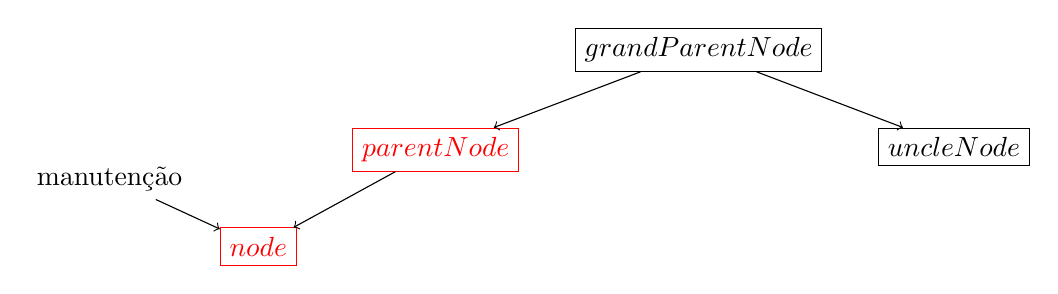
\begin{tikzpicture}
        \node[rectangle, draw, color = black] (gpNode) at (1, 1) {$grandParentNode$};
        \node[rectangle, draw, color = black] (uNode) [below right = 1cm of gpNode] {$uncleNode$};
        \node[rectangle, draw, color = red] (pNode) [below left = 1cm of gpNode] {$parentNode$};
        \node[rectangle, draw, color = red] (node) [below left = 1cm of pNode] {$node$};

        \node (m) [above left = 0.5cm of node] {manutenção};

        \draw (gpNode) edge[->] (pNode);
        \draw (gpNode) edge[->] (uNode);
        \draw (pNode) edge[->] (node);
        \draw (m) edge[->] (node);
      \end{tikzpicture}
    }
  }
  \subfigure[Depois da mudança de cores]{
    \scalebox{0.7}{
      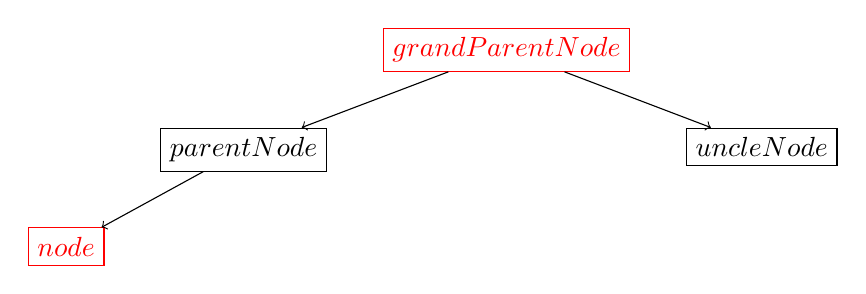
\begin{tikzpicture}
        \node[rectangle, draw, color = red] (gpNode) at (1, 1) {$grandParentNode$};
        \node[rectangle, draw, color = black] (uNode) [below right = 1cm of gpNode] {$uncleNode$};
        \node[rectangle, draw, color = black] (pNode) [below left = 1cm of gpNode] {$parentNode$};
        \node[rectangle, draw, color = red] (node) [below left = 1cm of pNode] {$node$};

        \draw (gpNode) edge[->] (pNode);
        \draw (gpNode) edge[->] (uNode);
        \draw (pNode) edge[->] (node);
      \end{tikzpicture}
    }
  }
  \subfigure[Depois da rotação]{
    \scalebox{0.7}{
      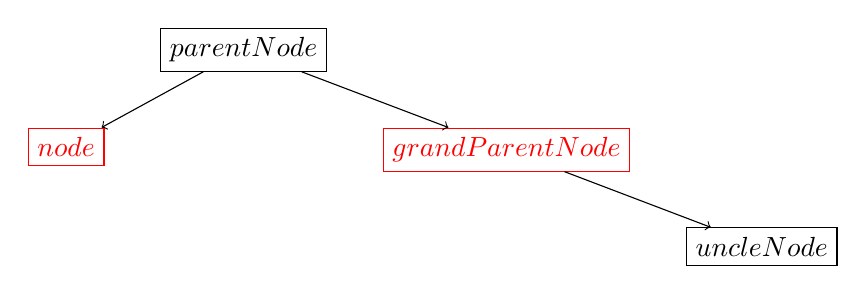
\begin{tikzpicture}
        \node[rectangle, draw, color = black] (pNode) at (1, 1) {$parentNode$};
        \node[rectangle, draw, color = red] (node) [below left = 1cm of pNode] {$node$};
        \node[rectangle, draw, color = red] (gpNode) [below right = 1cm of pNode] {$grandParentNode$};
        \node[rectangle, draw, color = black] (uNode) [below right = 1cm of gpNode] {$uncleNode$};

        \draw (pNode) edge[->] (node);
        \draw (gpNode) edge[->] (uNode);
        \draw (pNode) edge[->] (gpNode);
      \end{tikzpicture}
    }
  }
  \caption{Ilustração do caso 3 da inserção.}
\label{org52743c4}
\end{figure}

\begin{exercicio}
Argumente que, após uma inserção, é preciso fazer no máximo
duas rotações simples para manter as propriedades de uma Árvore
Rubro-Negra.
\end{exercicio}

\begin{exercicio}
Considere uma Árvore Rubro-Negra com \(n\) nós internos.
Argumente que, se \(n \geq 2\), então a árvore tem nós vermelhos.
\end{exercicio}

TODO Da próxima vez que lecionar a disciplina, tratar da remoção
em Árvores Rubro-Negras.
\end{enumerate}

\subsubsection{Implementação}
\label{sec:org94e6835}

Estruturalmente, a implementação de \texttt{RBTree} é análoga à
implementação de \texttt{AVLTree}, uma vez que ambas são subclasses de
\texttt{BSTree}.  Posto isso, e como iremos realizar a implementação de
\texttt{RBTree} em laboratório, inclusive de suas funções auxiliares, não
é necessária a apresentação de código-fonte.

\subsubsection{Análise de Complexidade}
\label{sec:org952238e}

Como sabemos, a complexidade das operações de uma Árvore Binária
de Busca é \(O(h)\), onde \(h\) é a altura da árvore.  Uma Árvore
Rubro-Negra com \(n\) nós internos tem altura \(h \in O(\log n)\).
Dessa forma, o custo de suas operações consiste do custo usual de
\(O(\log n)\) mais o custo de manutenção de suas propriedades, após
cada operação de modificação.

Sabemos que o custo de manutenção após uma operação de modificação
pode chegar a \(O(\log n)\).  Assim, o custo total das operações de
uma Árvore Rubro-Negra é \(O(\log n)\), ou seja, assintoticamente o
custo de melhor caso para modificações em Árvores Binárias de
Busca.

\subsection{Árvores B}
\label{sec:orgda04522}

Árvores B são árvores de busca balanceadas, usadas principalmente
em armazenamento secundário, como por exemplo sistemas de arquivos
de discos e bancos de dados.  São essencialmente uma generalização
de Árvores Binárias de Busca, em que é permitido a um nó ter mais
de uma chave.

Com um fator de ramificação \(bf\) (de \emph{branching factor})
possivelmente maior que o de uma Árvore Binária de Busca (\(bf \geq
   2\)) e usualmente determinado pelo tamanho de uma página de disco,
uma Árvore B com \(n\) nós deve ter altura \(O(\log_{bf} n)\).  Isso
permite que suas operações sejam realizadas em tempo \(O(\log n)\).

\subsubsection{Definição}
\label{sec:org72d625a}

Seja \(T\) uma Árvore B. As seguintes propriedades devem ser
satisfeitas por \(T\):
\begin{itemize}
\item cada \(node\) de \(T\) tem os seguintes atributos:
\begin{itemize}
\item \(node.n\), o número de chaves armazenadas em \(node\);
\item as chaves \(node.key_1, node.key_2, \dots, node.key_n\),
armazenadas de forma que \(node.key_1 \leq node.key_2 \leq
        \dots \leq node.key_n\);
\item Um campo booleano \(node.leaf\), indicando se \(node\) é uma
folha.
\end{itemize}
\item cada \(node\) com \(node.leaf\) falso deve ter \(node.n + 1\)
sub-árvores \(node.subtree_1, node.subtree_2\), \(\dots,
      node.subtree_{n + 1}\);
\item para cada \(node\) com \(node.leaf\) falso, e para qualquer chave
\(k_i\) da sub-árvore \(node.subtree_i\), para \(1 \leq i \leq
      node.n + 1\), temos \(k_1 \leq node.key_1 \leq k_2 \leq node.key_2
      \leq \dots \leq k_n \leq node.key_n \leq k_{n + 1}\);
\item todo \(node\) com \(node.leaf\) verdadeiro está no mesmo nível, e
esse nível é justamente a altura de \(T\);
\item cada \(node\) tem \(node.n\) limitado, tanto inferior como
superiormente.  Isso significa que, dado \(t \geq 2\):
\begin{itemize}
\item cada \(node\), a menos da raiz, deve ter \(node.n \geq t - 1\), e
portanto deve ter no mínimo \(t\) sub-árvores;
\item cada \(node\) deve ter \(node.n \leq 2t - 1\), e portanto deve ter
no máximo \(2t\) sub-árvores.  Se \(node\) tem \(node.n = 2t - 1\),
dizemos que \(node\) está cheio.
\end{itemize}
\end{itemize}

\begin{theorem}
Tome uma Árvore B com \(n\) chaves, \(t \geq 2\) e altura \(h\).  Temos
$$
    h \leq \log_t\left( \frac{n + 1}{2} \right)
    $$
\end{theorem}

\begin{proof}
A raiz de uma Árvore B contém no mínimo uma chave, enquanto os
demais nós contém no mínimo \(t - 1\) chaves.  Assim, haveria a raiz
no nível 0, ao menos dois nós no nível 1, ao menos \(2t\) nós no
nível 2, ao menos \(2t^2\) nós no nível 3, e assim por diante, até
termos ao menos \(2t^{h - 1}\) nós no nível \(h\).  Com isso, temos
\begin{align}
n \geq&\, 1 + (t - 1)\sum_{i = 1}^{h} 2t^{i - 1} \\
     =&\, 1 + (t - 1)\left( 2\left( \frac{t^h - 1}{t - 1} \right) \right) \\
     =&\, 1 + 2(t^h - 1) \\
     =&\, 1 + 2t^h - 2 \\
     =&\, 2t^h - 1
\end{align}
A partir de \(n \geq 2t^h - 1\), temos \(t^h \leq \frac{n + 1}{2}\).
Basta tomar \(\log_t\) de ambos os lados dessa inequação para
concluir a prova.
\end{proof}

\begin{exercicio}
Em função de \(h\) e \(t\), qual o número máximo de chaves que uma
Árvore B de altura \(h\) e parâmetro \(t\) pode conter? E o mínimo?
\end{exercicio}

\subsubsection{Operações}
\label{sec:org83052d6}

Uma Árvore B suporta as operações usuais de busca, inserção e
remoção.  Dessas três, trataremos da remoção como uma atividade de
laboratório.  Dessa forma, definimos aqui a implementação de uma
Árvore B com as operações de busca e inserção, além de algumas
funções auxiliares.  Vamos apresnetar e descrever o conteúdo de
\texttt{btree.hpp}.

\begin{minted}[,fontsize=\footnotesize]{c++}
#pragma once

// array type
#include <array>
// smart pointers
#include <memory>
// optional type
#include <optional>

// generic b tree
template<typename Key, typename Val, unsigned int t>
class BTree{
  // ...
};
\end{minted}

Em \texttt{btree.hpp}, o único cabeçalho novo é \texttt{array}, que diferente de
\texttt{vector}, implementa um array de tamanho estático.  A classe
\texttt{BTree} será nossa implementação de Árvore B, e ela tem três
parâmetros: os tipos \texttt{Key} e \texttt{Val}, com seu significado usual; o
inteiro não-negativo \texttt{t}, fazendo jus à definição de que uma
página de \texttt{BTree} (a menos da raiz) deve ter entre \texttt{t - 1} e \texttt{2t -
    1} chaves.

\begin{minted}[,fontsize=\footnotesize]{c++}
private:
  // represents a page of BTree
  struct Page{
    // indicates whether page is a leaf
    bool leaf;
    // number of keys currently stored
    unsigned int numberKeys;
    // arrays of keys and vals
    std::array<Key, 2*t - 1> key;
    std::array<Val, 2*t - 1> val;
    // children array
    std::array<std::unique_ptr<Page>, 2*t> child;
    // constructor
    Page() : leaf{false},
             numberKeys{0},
             key{},
             val{},
             child{}
    {}
    // returns whether page is full
    bool isFull(){
      return numberKeys == 2*t - 1;
    }
    // searches for Key. In case it is not present, returns nothing
    std::optional<Val> search(Key k){
      // ...
    }
    // splits a full child of this node, if this node is nonfull.  In
    // case child index is invald or the former conditions are not
    // met, returns false
    bool splitChild(unsigned int childIndex){
      // ...
    }
  };
// ...
\end{minted}

Como primeiro membro privado de \texttt{BTree}, temos \texttt{Page},
representando uma página de uma árvore B.  Seu membro \texttt{leaf}
indica se a página é uma folha, enquanto \texttt{numberKeys} é o número
de chaves atualmente nela armazenadas.  Os membros \texttt{key} e \texttt{val}
armazenam chaves e valores correspondentes em posições de mesmo
índice.  Caso a página não seja uma folha, \texttt{child} deve armazenar
ponteiros para suas páginas filhas.  Note que as dimensões de
\texttt{key}, \texttt{val} e \texttt{child} estão de acordo com a definição de uma
Árvore B.

Quanto aos métodos de \texttt{Page}, o construtor não inspira muitos
comentários.  A função \texttt{isFull} determina se a página está cheia,
e isso ocorre quando o número de chaves nela armazenada é
exatamente o número de posições de \texttt{key}.  O método \texttt{search} é
autodescritivo em sua finalidade, e \texttt{splitChild} divide um filho
cheio de uma página não-cheia em dois.

\begin{minted}[,fontsize=\footnotesize]{c++}
std::optional<Val> search(Key k){
  unsigned int i = 0;
  // we go right searching for k
  while (i < numberKeys && k > key[i]){
    i++;
  }
  // now either key[i - 1] < k <= key[i] or i > numberKeys - 1
  // if k was found, we return the corresponding value
  if (i < numberKeys && k == key[i]){
    return val[i];
  }
  // now either key[i - 1] < k < key[i] or i > numberKeys - 1.  In
  // either case, we need to either go down or report an failed
  // search
  // if this page is a leaf, there is nowhere to go down, and the
  // search fails
  else if (leaf){
    return {};
  }
  // otherwise, we recurse into the appropriate child
  else{
    return child[i]->search(k);
  }
}
\end{minted}

A função \texttt{search} admite que as chaves estão armazenadas em ordem
crescente, e assim faz \texttt{i} assumir o menor índice tal que \texttt{k <=
    key[i]}.  Caso \texttt{k == key[i]}, a chave buscada é encontrada, e
\texttt{val[i]} é retornado.  Caso contrário, sabe-se que \texttt{k < key[i]}, e
portanto a chave pode se encontrar no filho ``esquerdo'' de
\texttt{key[i]}, \texttt{child[i]}, onde a busca é feita recursivamente.

Há ainda as situações em que a página é uma folha e em que \texttt{k} é
maior que todas as chaves da página.  No primeiro cenário, se \texttt{k}
não estiver presente na página, a busca encerra retornando nada.
No segundo, note que \texttt{i == numberKeys}, e \texttt{k} pode se encontrar no
filho ``direito'' de \texttt{key[numberKeys - 1]}, \texttt{child[numberKeys]}.

\begin{exercicio}
Desenvolva algoritmos para encontrar as chaves mínima e máxima de
sub-árvores de uma Árvore B.  Desenvovla também algoritmos para
encontrar as chaves sucessora e predecessora de uma certa chave.
\end{exercicio}

\pagebreak

\begin{minted}[,fontsize=\footnotesize]{c++}
bool splitChild(unsigned int childIndex){
  if (!isFull() && childIndex <= numberKeys && child[childIndex]->isFull()){
    // ...
  }
  else{
    return false;
  }
}
\end{minted}

Antes de realizar sua operação, \texttt{splitChild} verifica se a página
não está cheia, se \texttt{childIndex} é índice de algum filho da página
e, por fim, se o referido filho se encontra cheio.  Caso uma
dessas condições não seja atendida, \texttt{splitChild} apenas sinaliza
que sua operação não ocorreu.

\pagebreak

\begin{minted}[,fontsize=\footnotesize]{c++}
if (!isFull() && childIndex <= numberKeys && child[childIndex]->isFull()){
  // a reference to the child to be split
  auto& splittingChild = child[childIndex];
  // its new "right" sibling
  std::unique_ptr<Page> newSibling = std::make_unique<Page>();
  // newSibling is a leaf iff splittingChild is a leaf
  newSibling->leaf = splittingChild->leaf;
  newSibling->numberKeys = t - 1;
  for (unsigned int i = 0; i < t - 1; i++){
    newSibling->key[i] = splittingChild->key[t + i];
    newSibling->val[i] = splittingChild->val[t + i];
  }
  // if newSibling is not a leaf, it also receives some
  // children from splittingChild
  if (!newSibling->leaf){
    for (unsigned int i = 0; i < t; i++){
      newSibling->child[i] = std::move(splittingChild->child[t + i]);
    }
  }
  splittingChild->numberKeys = t - 1;
  // we make room for newSibling at position childIndex + 1 ...
  for (unsigned int i = numberKeys; i >= childIndex + 1; i--){
    child[i + 1] = std::move(child[i]);
  }
  // ... and put it right there
  child[childIndex + 1] = std::move(newSibling);
  // now we make room for the median key (and its val) of splittingChild at
  // position childIndex of this node ...
  if (numberKeys > 0){
    for(unsigned int i = numberKeys - 1; i >= childIndex; i--){
      key[i + 1] = key[i];
      val[i + 1] = val[i];
    }
  }
  // ... and put it right there
  key[childIndex] = splittingChild->key[t - 1];
  val[childIndex] = splittingChild->val[t - 1];
  // and this page just gained a new key
  numberKeys++;
  return true;
}
\end{minted}

Caso suas condições sejam atendidas, \texttt{splitChild} cria o novo
irmão ``direito'' de \texttt{splittingChild}, \texttt{newSibling}.  Como ficarão
no mesmo nível, \texttt{newSibling} é folha sse \texttt{splittingChild} é folha.

Após isso, as \texttt{2*t - 1} chaves de \texttt{splittingChild} (que está
cheio) são remanejadas: as \texttt{t - 1} menores chaves permanecem em
\texttt{splittingChild}; as \texttt{t - 1} maiores ficam com \texttt{newSibling}; a
chave mediana fica com seu pai, justamente para fazer a
``separação'' entre \texttt{splittingChild} e \texttt{newSibling}.  Caso
\texttt{splittingChild} tenha filhos, os filhos correspondentes às chaves
movidas para \texttt{newSibling} também são dados a \texttt{newSibling}.

Em relação ao pai, note que é preciso posicionar adequadamente
tanto a chave mediana recebida de \texttt{splittingChild} quanto
\texttt{newSibling} (entre seus filhos).  Para isso, chaves e filhos
sofrem um \emph{shift} para a direita (possível porque o pai não está
cheio), de forma que a chave mediana de \texttt{splittingChild} possa se
tornar \texttt{key[childIndex]} (\texttt{splittingChild} torna-se filho
``esquerdo'' de sua antiga chave mediana) e \texttt{newSibling} possa se
tornar \texttt{child[childIndex + 1]} (\texttt{newSibling} torna-se filho
``direito'' da antiga chave mediana de \texttt{splittingChild}).

\begin{minted}[,fontsize=\footnotesize]{c++}
private:
  // ...
  // root pointer
  std::unique_ptr<Page> root;
public:
  // constructor
  BTree() : root{nullptr}
  {}
  bool isEmpty(){
    return root == nullptr;
  }
  // search method
  std::optional<Val> search(Key key){
    if (root){
      return root->search(key);
    }
    else{
      return {};
    }
  }
  // ...
\end{minted}

Por enquanto, estamos omitindo um membro privado, mas listamos
\texttt{root}, o ponteiro para a página raiz de \texttt{BSTree}.  Os membros
públicos dessa listagem são bastante triviais.

\pagebreak

\begin{minted}[,fontsize=\footnotesize]{c++}
// ...
public:
  // ...
  // insert method
  bool insert(Key key, Val val){
    // if key is present we just signal insertion did not occur
    if (search(key)){
      return false;
    }
    // otherwise we do the insertion
    else{
      // if tree is not empty
      if (root){
        // if root is full ...
        if (root->isFull()){
          // ... we create a new root, ...
          std::unique_ptr<Page> newRoot = std::make_unique<Page>();
          // ... make it the parent of the old root, ...
          newRoot->child[0] = std::move(root);
          // ... update root pointer, ...
          root = std::move(newRoot);
          // and split the old root
          root->splitChild(0);
        }
        // here root is certain to be nonfull, so we make the insertion
        insertOnNonfullPage(root.get(), key, val);
      }
      // if there is no root
      else{
        // we make a new one ...
        root = std::make_unique<Page>();
        // ... which is surely a leaf ...
        root->leaf = true;
        // ... and then we perform the insertion
        insertOnNonfullPage(root.get(), key, val);
      }
      // in either case, insertion took place
      return true;
    }
  }
\end{minted}

O método \texttt{insert}, antes de tudo, verifica se a árvore já contém a
chave a ser inserida.  Em caso afirmativo, a inserção não ocorre e
isso é sinalizado.  Caso contrário, verifica-se se a raiz é nula.
Nessa situação, a inserção vai criar a página raiz, que certamente
não está cheia, tratá-la como folha e usar \texttt{insertOnNonfullPage}
(a ser apresentada) para realizar a inserção.

Caso já haja uma raiz, verificamos se ela está cheia.  Caso
esteja, criamos uma nova página como pai da raiz, e a dividimos
com o \texttt{splitChild} da nova página, que passa a ser nossa nova
raiz.  Como a nova raiz tem exatamente uma página e \texttt{t >= 2}, a
nova raiz não está cheia, e após isso fazemos a inserção com
\texttt{insertOnNonfullPage} na raiz da árvore.  Agora apresentamos
\texttt{insertOnNonfullPage}.

\begin{exercicio}
Explique por que uma Árvore B tem sua altura aumentada apenas
quando sua raiz é dividida.
\end{exercicio}

\pagebreak

\begin{minted}[,fontsize=\footnotesize]{c++}
// inserts key val pair on nonfull page
static void insertOnNonfullPage(Page* page, Key key, Val val){
  // index of "rightest" key
  int i = page->numberKeys - 1;
  // if page is a nonfull leaf, we do the insertion
  if (page->leaf){
    // while we search for the appropriate place to put key and val,
    // we also make room for them
    while (i >= 0 && key < page->key[i]){
      page->key[i + 1] = page->key[i];
      page->val[i + 1] = page->val[i];
      i--;
    }
    // we put key and val into their appropriate places ...
    page->key[i + 1] = key;
    page->val[i + 1] = val;
    // ... and update numberKeys
    page->numberKeys++;
  }
  // if page is not a leaf, we recurse to its appropriate child
  else{
    // looking for the child index to recurse
    while (i >= 0 && key < page->key[i]){
      i--;
    }
    // when we exit the while loop,
    // page->key[i] <= key < page->key[i+1], so insertion will
    // recurse into page->child[i + 1]
    i++;
    // before going down, we verify whether page->child[i] is full.
    // In case it is, we split it ...
    if (page->child[i]->isFull()){
      page->splitChild(i);
      // ... and see if the insertion should take place in the newly
      // created sibling, that is, we see if key is greater than the
      // median key that just went up from page->child[i] to page
      if (key > page->key[i]){
        i++;
      }
    }
    // finally, we perform the recursive insertion
    insertOnNonfullPage(page->child[i].get(), key, val);
  }
}
\end{minted}

A função \texttt{insertOnNonfullPage} trata de forma distinta folhas e
não-folhas.  Quando recebe uma folha, e essa deve ser não-vazia,
apenas é realizado um \emph{shift} para a direita para que a chave a
ser inserida seja posta em seu devido lugar, mantendo as chaves da
página em ordem crescente.

Quando se trata da inserção em uma não-folha, a operação é feita
recursivamente em um de seus filhos.  Após determinado em que
filho deve ser realizada a inserção, é preciso verificar se ele
está cheio. Caso não esteja, a operação recursiva é realizada
imediatamente.  Mas se estiver cheio, esse filho precisa ser
dividido em dois filhos não-cheios. Após isso, é preciso comparar
a chave a ser inserida com a chave mediana que acabou de ``subir''
para o pai, e baseado nessa comparação, decide-se em qual dos dois
novos filhos deve ser feita a inserção.

Com a definição de \texttt{insertOnNonfullPage}, notamos que novas chaves
são sempre inseridas em folhas.  As páginas que não são folhas
ganham novas chaves apenas quando a chave mediana de um de seus
filhos ``sobe''.  É possível observar também que, no caminho da
raiz até a folha em que a inserção irá ocorrer,
\texttt{insertOnNonfullPage} divide todas as páginas cheias que encontra.

\begin{exercicio}
Qual a complexidade do procedimento de inserção para uma Árvore B
de altura \(h\) e parâmetro \(t\)?
\end{exercicio}

Agora lidamos com a operação de remoção.  Como esta vai ser
passada como atividade de laboratório, vamos apenas descrever seu
funcionamento, sem a apresentação de código-fonte.

Baseando-se na invariante de que \texttt{page} sempre terá mais que \texttt{t -
    1} chaves (a menos que seja a raiz), podemos descrever o
procedimento de remoção com os seguintes casos:
\begin{enumerate}
\item estamos removendo \texttt{key} de uma \texttt{page} não-folha:
\begin{enumerate}
\item que não contém \texttt{key}: considerando \texttt{0 <= j < numberKeys}, se
\texttt{key} é maior que toda \texttt{key[j]}, fazemos \texttt{i = numberKeys};
se \texttt{key} é menor que toda \texttt{key[j]}, fazemos \texttt{i = 0}; do
contrário, fazemos \texttt{i} ser tal que \texttt{key[i - 1] < key <
          key[i]}; uma vez definido \texttt{i}, a sub-árvore enraizada em
\texttt{child[i]} pode conter \texttt{key}:
\begin{enumerate}
\item \texttt{child[i]} tem mais que \texttt{t - 1} chaves: recursivamente,
removemos \texttt{key} de \texttt{child[i]};
\item \texttt{child[i]} tem \texttt{t - 1} chaves:
\begin{enumerate}
\item \label{org4e81f98} \texttt{child[i]} tem um
irmão adjacente (\texttt{child[i - 1]} ou \texttt{child[i + 1]}) com
mais que \texttt{t - 1} chaves: caso esse seja \texttt{child[i -
                1]}, movemos sua maior chave para o lugar de \texttt{key[i -
                1]}, que se torna a menor chave de \texttt{child[i]} (após um
\emph{shift} para a ``direita'' nas chaves e nos filhos de
\texttt{child[i]}); o filho mais ``à direita'' de \texttt{child[i -
                1]} torna-se o filho de índice \texttt{0} de \texttt{child[i]};
temos um procedimento análogo para \texttt{child[i + 1]};
\item \label{orgdfb958d} \texttt{child[i]} não tem irmãos
adjacentes com mais que \texttt{t - 1} chaves: vamos supor
que \texttt{child[i - 1]} é um filho válido de \texttt{page}; como
\texttt{child[i - 1]} e \texttt{child[i]} têm \texttt{t - 1} chaves cada,
fazemos o \emph{merge} de \texttt{child[i - 1]}, \texttt{key[i - 1]} e
\texttt{child[i]}, e colocamos a página resultante (com \texttt{2t -
                1} chaves) em \texttt{child[i - 1]}; fazemos um \emph{shift} para
a ``esquerda'' nas chaves de \texttt{page}, de \texttt{key[i]} em
diante, e nos filhos de \texttt{page}, de \texttt{child[i + 1]} em
diante; há um procedimento análogo para \texttt{child[i +
                1]}, caso \texttt{child[i - 1]} não seja um filho válido;
\end{enumerate}
\end{enumerate}
\item que contém \texttt{key} como \texttt{key[i]}:
\begin{enumerate}
\item caso \texttt{child[i]} tenha mais que \texttt{t - 1} chaves:
encontramos o predecessor de \texttt{key} em \texttt{child[i]}, digamos
\texttt{predKey}; sobrescrevemos \texttt{key} com \texttt{predKey} e
deletamos, recursivamente, \texttt{predKey} de \texttt{child[i]};
\item caso \texttt{child[i + 1]} tenha mais que \texttt{t - 1} chaves:
análogo ao caso anterior, mas em relação ao sucessor de
\texttt{key} em \texttt{child[i + 1]};
\item \label{org59412f0} caso ambos \texttt{child[i]} e
\texttt{child[i + 1]} tenham \texttt{t - 1} chaves: os números de
chaves e de filhos de \texttt{page} diminuem em 1 quando fazemos
o \emph{merge} de \texttt{child[i]}, \texttt{key[i]} e \texttt{child[i + 1]},
criando um novo filho de \texttt{page} com \texttt{2t - 1} chaves que
será \texttt{child[i]}; as chaves de \texttt{key[i + 1]} em diante
sofrem um \emph{shift} para a ``esquerda''; agora podemos
remover \texttt{key} de \texttt{child[i]};
\end{enumerate}
\end{enumerate}
\item estamos removendo \texttt{key} de uma \texttt{page} folha:
\begin{enumerate}
\item que não contém \texttt{key}: neste caso, sabemos que a árvore não
contém \texttt{key}, e portanto nenhuma chave é removida;
\item que contém \texttt{key}: removemos \texttt{key} de \texttt{page}; caso \texttt{page} não
seja raiz, a invariante garante que \texttt{page} tem agora pelo
menos \texttt{t - 1} chaves.
\end{enumerate}
\end{enumerate}

\begin{exercicio}
Qual a complexidade do procedimento de remoção para uma Árvore B
de altura \(h\) e parâmetro \(t\)?
\end{exercicio}

\pagebreak

\section{Laboratórios}
\label{sec:orgbc802ad}

Nesta seção, descrevemos atividades práticas que devem ser
desenvolvidas em aulas de laboratório.  Idealmente, deve haver uma
subseção para cada estrutura de dados descrita nestas notas de aula.

\subsection{Árvores Binárias de Busca}
\label{sec:orga596f7c}

Neste laboratório, vamos desenvolver atividades majoritariamente
relacionadas com passeios em Árvores Binárias de Busca.

\begin{enumerate}
\item Implemente os seguintes métodos na classe \texttt{BSTree} como
públicos:
\begin{enumerate}
\item \texttt{static std::vector<std::pair<Key, Val>> inOrder(const BSTree<Key, Val>\& bst)}
\item \texttt{static std::vector<std::pair<Key, Val>> preOrder(const BSTree<Key, Val>\& bst)}
\item \texttt{static std::vector<std::pair<Key, Val>> postOrder(const BSTree<Key, Val>\& bst)}
\end{enumerate}
Lembramos que, como esses métodos não devem alterar a \texttt{BSTree}
passada como argumento, todos eles receben uma referência
\texttt{const} para \texttt{BSTree}.  Caso tivéssemos, por exemplo, um objeto
\texttt{bst} de tipo \texttt{BSTree<int, char>}, faríamos a chamada
\texttt{BSTree<int, char>::inOrder(bst)}.
\item Implemente o método \texttt{bool update(Key key, Val newVal)} como
público em \texttt{BSTree}.  O método dever retornar \texttt{false} sse \texttt{key}
não está presente na árvore.
\item Escreva testes em \texttt{bstree\_test.cpp} para assegurar que a
implementação de seus métodos está correta.
\item Escreva um programa em \texttt{lab1.cpp} que, dado o nome de um
arquivo, imprime no terminal o número de ocorrências de palavras
no arquivo (se a palavra ``gato'' ocorre três vezes, o programa
deve imprimir a linha \texttt{gato: 3} ou algo próximo disso). O
programa deve imprimir as palavras em ordem alfabética.  Dica:
use uma \texttt{BSTree<std::string, int>}.
\item Por fim, crie uma ``receita'' em \texttt{makefile} de forma que o
executável \texttt{lab1} possa ser construído com o comando \texttt{make
      lab1}.
\end{enumerate}

\subsection{Árvores AVL}
\label{sec:org75cd03a}

Neste laboratório, nosso objetivo é completar a implementação de
\texttt{AVLTree}, conforme as indicações feitas na Subseção \ref{org6ea5e87}.  Além
disso, vamos escrever testes para garantir que nossa implementação
está correta.

\begin{enumerate}
\item Existe uma rotação já implementada, \texttt{rotateR} (rotação simples à
direita).  Implemente as outras três rotações (\texttt{rotateL},
\texttt{rotateLR} e \texttt{rotateRL}), também como métodos estáticos privados
de \texttt{AVLTree}.  As rotações duplas poderiam ser definidas em
termos das rotações simples?
\item Complete a implementação de \texttt{rebalanceNode}, utilizando chamadas
para as rotações nos casos adequados.
\item Complete a implementação de \texttt{insert}, utilizando
\texttt{pathToExistingKey} (herdado de \texttt{BSTreeWithNode}),
\texttt{updateHeightsOnPath} e \texttt{rebalanceNodesOnPath}.  Lembre-se que
os nós que precisam ser verificados formam um caminho da raiz
até o nó recém-inserido.
\item Faça o mesmo para \texttt{remove}.  Dessa vez, o caminho de nós que
precisa de manutenção vai da raiz até o pai do nó excluído.
\item Acrescente um método público \texttt{isBalanced} a \texttt{AVLTreeWithNode},
que existe apenas quando \texttt{checkBalance} está definido.  Para
isso, use as diretivas de pré-processamento \texttt{\#ifdef} e \texttt{\#endif}.
O objetivo de \texttt{isBalanced} é verificar se cada \(node\) satisfaz
\(balance(node) \in \{-1, 0, 1\}\).  Não se esqueça de criar um
método público \texttt{isBalanced} em \texttt{AVLTree} (que existe apenas com
\texttt{checkBalance} definido) que redireciona sua chamada para o
\texttt{isBalanced} de \texttt{avlt}.
\item Agora que todos os métodos estão completos e que temos
ferramentas para teste, escreva mais testes em
\texttt{avltree\_test.cpp}, de forma a garantir que sua implementação de
fato mantém a árvore bem balanceada.  Use \texttt{\#define checkBalance}
(antes de incluir \texttt{avltree.hpp}) em \texttt{avltree\_test.cpp} para
tornar \texttt{isBalanced} disponível, e chame-o em um \texttt{assert} após
cada operação de modificação em seus testes.
\end{enumerate}

\subsection{Árvores Rubro-Negras}
\label{sec:orgef057c7}

O objetivo deste laboratório é completar o código-fonte de
\texttt{RBTree}, seguindo as indicações feitas em \texttt{rbtree.hpp}.  Algumas
funções auxiliares serão sugeridas, tanto para facilitar a
implementação como para a realização de testes.

\begin{enumerate}
\item Vamos tratar \texttt{nullptr} como nossas folhas pretas sem dados
significativos.  Implemente os seguintes métodos privados em
\texttt{RBTree}:
\begin{itemize}
\item \texttt{static Color color(const std::unique\_ptr<RBTreeNode>\& node);}
\item \texttt{static Color color(const std::nullptr\_t nptr);}
\end{itemize}
A especialização de \texttt{color} para \texttt{std::nullptr\_t} deve sempre
retornar \texttt{Color::black}.  Assim, usaremos esse método para
determinar a cor de um nó, mesmo que ele seja \texttt{nullptr}.
\item Implemente as funções de rotação simples como métodos privados
de \texttt{RBTRee}:
\begin{itemize}
\item \texttt{static void rotateR(RBTreeNode* node);}
\item \texttt{static void rotateL(RBTreeNode* node);}
\end{itemize}
É possível basear-se nas rotações simples de \texttt{AVLTree}.
\item Implemente a função \texttt{static void
      insertionMaintenance(RBTreeNode* node)} como método privado de
\texttt{RBTree}.  Essa função deve sempre ser chamada com nós
vermelhos, já que a manutenção é sempre feita para nós
vermelhos.  O propósito dessa função é fazer as trocas de cor e
rotações necessárias para manter as propriedades de um nó de
\texttt{RBTree} após uma inserção.  O método \texttt{pathToExistingKey} pode
ser útil para essa função.
\item Complete a implementação de \texttt{insert} com a operação de
manutenção para o nó recém-inserido.  O que deve ser feito para
tomar um ponteiro para esse nó?
\item Acrescente o método público \texttt{bool obeysProperties()} a
\texttt{RBTreeWithNode} (e também a \texttt{RBTree}), que deve existir apenas
quando \texttt{checkProperties} estiver definido.  O objetivo de
\texttt{obeysProperties} é verficar se \texttt{RBTree} satisfaz as
propriedades de uma Árvore Rubro-Negra.
\item Acrescente mais testes a \texttt{rbtree\_test.cpp}, de forma a garantir
que sua implementação de \texttt{RBTree} está correta.  Use \texttt{\#define
      checkProperties} (antes de incluir \texttt{rbtree.hpp}) de forma a
tornar \texttt{obeyProperties} disponível.  Após cada operação de
modificação em seus testes, chame \texttt{obeyProperties} em um
\texttt{assert}.
\end{enumerate}

\subsection{Árvores B}
\label{sec:org3a7f709}

A finalidade deste laboratório é completar o código-fonte de
\texttt{BTree}, seguindo as indicações feitas em \texttt{btree.hpp}.  A principal
atividade aqui proposta é a implementação do método \texttt{remove} de
\texttt{BTree}, a ser seguida pela realização de testes que assegurem o
funcionamento correto de \texttt{BTree}.

\begin{enumerate}
\item Implemente os métodos \texttt{rotateKeysL} e \texttt{rotateKeysR} de \texttt{Page}.
Esses métodos estão relacionados com o caso
\ref{org4e81f98} da remoção.
\item Implemente o método \texttt{mergeSiblingsWithKey} de \texttt{Page}.  Note que
esse método é utilizado nos casos \ref{orgdfb958d} e
\ref{org59412f0} da remoção.
\item Implemente o método \texttt{remove} de \texttt{BTree}.  As funções dos pontos
anteriores podem ser úteis nessa implementação.
\item Em \texttt{btree\_test.cpp}, acrescente chamadas de inserção, busca e
remoção.  Após cada operação de modificação, verifique (com
\texttt{assert}) se as chaves contidas na árvore estão associadas aos
seus devidos valores.
\end{enumerate}
\end{document}